\chapter*{Introduction}
\addcontentsline{toc}{chapter}{Introduction}

\section*{Context}
%%% CONTEXT
\malettrine{P}{roviding} decisional autonomy to a robot 
requires among other things to compute a function which returns
the symbols of the actions to be triggered
at a given moment, considering the data from its sensors.
The features of interest of the robot 
and its  surroundings form a \textit{system}.
In general, for a given sequence of actions performed by the robot, 
the evolution of this system 
is not fixed for sure, 
but its behavior may be known 
by performing tests on the robot
or using information from expert knowledge.
As well, the raw or processed data from the robot sensors
are not generally a deterministic outcome
of the state of the system or of the taken actions:
nevertheless, these data, 
called also \textit{observations} of the system, 
depend on the robot's actions and system states. 
Relations between observations, system states and actions 
may be known through tests of the sensors
in various situations, 
or by taking into account the description of the sensors, 
data processing, or any related expert information.
For instance, in the case of a robot using Computer Vision (CV),
the output of the image processing algorithm employed
is considered as an observation of the system
since it is the result of processed sensor data
and the input of the decision model:
here data are images from camera.
For a given camera, and a given vision algorithm,
the behavior of the observation
is related to the action and to the system state
during the process of taking images. 

Thus, in order to make a robot 
autonomously fulfill a chosen \textit{mission}, 
we are  looking for a function returning actions 
conditioned on the sequence of system observations,
and taking into account uncertainty 
about the system evolution 
and its observation.
Such functions may be called \textit{strategies}.
The research domain associated to this kind of problem,
\textit{i.e.} strategy computation,
is not restricted to robotics and
is called \textit{sequential decision making under uncertainty}:
in the general case,
the entity which has to act is called the \textit{agent}.
In this thesis, although provided results are mostly theoretical
and general enough to tackle much more various applications,
the problem of strategy computation 
is studied in the context of autonomous robotics,
and the agent is the decisional part of the robot.
Computing a strategy for a given robotic mission needs a proper framework:
the best known model describes the state and observation behaviors
using Probability Theory.

\subsection*{A probabilistic model for strategy computation}

Markov Decision Processes (MDPs) 
define a useful formalism 
to express sequential decision problems 
under probabilistic uncertainty \cite{Bel}.
It is a framework well suited to compute strategies 
if the actual system state is known by the agent
at each point in time.
In the robotic context,
this assumption means that
the considered mission allows us to assume 
that the robot has full knowledge 
of the features of interest via its sensors.
In this model,
a system state is denoted by the letter $s$,
and the finite set of all the possible states is $\mathcal{S}$.
The finite set $\mathcal{A}$ consists
of all possible actions $a \in \mathcal{A}$ 
available to the agent. 
The time is discretized into integers $t \in \mathbb{N}$
which represent time steps of the action sequence.

The state dynamics is assumed to be \textit{Markovian}:
at each time step $t$,
the next system state $s_{t+1} \in \mathcal{S}$,  
only depends on the current one $s_t \in \mathcal{S}$
and the chosen action $a_t \in \mathcal{A}$.
This relation is described by a transition function 
$\textbf{p} \paren{ s_{t+1} \sachant s_t, a_t}$
which is defined as the probability distribution %%%% TODO TODO TODO TODO
on the next system states $s_{t+1}$ conditioned on each action: 
if the action $a_t \in \mathcal{A}$ is selected by the agent, 
and the current system state is $s_t \in \mathcal{S}$, 
the next state $s_{t+1} \in \mathcal{S}$
is reached with probability $\textbf{p} \paren{ s_{t+1} \sachant s_t, a_t }$. 

The mission of the agent is described in terms of rewards:
a reward function $r: (s,a) \mapsto r(s,a) \in \mathbb{R}$ 
is defined for each action $a \in \mathcal{A}$
and system state $s \in \mathcal{S}$,
and models the goal of the agent.
Each reward value $r(s,a) \in \mathbb{R}$
is a local incentive for the agent.
The more rewards are gathered during one execution of the process, the better:
a realization of a sequence of system states
and actions is considered as well fulfilling the desired mission 
if encountered rewards $r(s_t,a_t)$ are high.
Solving an infinite horizon MDP
consists in computing an optimal strategy, 
\textit{i.e.} a function prescribing actions $a \in \mathcal{A}$
to be taken over time,
and maximizing the mean
of the sum of rewards gathered during one execution:
this mean is computed with respect to the probabilistic behavior of the system state
encoded by transition functions $\textbf{p} \paren{s_{t+1} \sachant s_t,a_t}$.
For instance, a preferred strategy 
may be a function $d$ defined on $\mathcal{S}$,
as the current state is available to the agent, 
and with values in $\mathcal{A}$.

%%% ROBOT POMPIER
\begin{figure} \centering
\definecolor{ggreen}{rgb}{0.3,0.7,0.4}
\begin{tikzpicture}
\node (rpomp) at (-1,4.7) {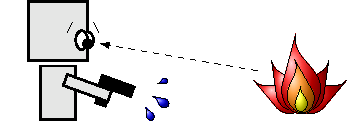
\includegraphics[scale=0.9]{robot_pompier}};
\node (bli) at (0,6.5) {};
\node (pomdp3) at (3.9,6) {\color{orange}{$s \in \mathcal{S}$}: \color{black}{\textbf{system state}}};
\node (t1) at (2,6) {};
\node (r1) at (-2.3,5.5) {};
\node (r11) at (1,4.5) {};
\draw[->,>=latex,color=orange!60,line width=1mm] (t1) to (r1);
\draw[->,>=latex,color=orange!60,line width=1mm] (t1) to (r11);
\node (pomdp4) at (5.8,4.45) {\color{blue!60}{$o \in \mathcal{O}$:} \color{black} \textbf{system observation}};
\node (t2) at (3.3,4.4) {};
\node (r2) at (-2.3,5.05) {};
\draw[->,>=latex,color=blue!40,line width=1mm] (t2) to[bend left] (r2);
\node (pomdp5) at (1.8,3) {\color{red}{$a \in \mathcal{A}$:} \color{black} \textbf{agent's action}};
\node (t3) at (-0.3,3) {};
\node (r3) at (-2,4.2) {};
\draw[->,>=latex,color=red!50,line width=1mm] (t3) to (r3);
\node (pomdp6) at (-5.5,5.5) {\color{ggreen}{$b \in \mathbb{P}^{\mathcal{S}}$:} \color{black} \textbf{belief state} }; %%% ORANGE?
\node (pomdp6) at (-3.5,6) {\color{ggreen}{\Huge \textbf{?}}}; %%% ORANGE?
\end{tikzpicture}
\caption[Use of a POMDP for the firefighter robot mission modeling]{
Use of a POMDP for the firefighter robot mission modeling:
in this toy example, the mission of the robot is fire prevention.
The \textbf{states of the system} $s�\in \mathcal{S}$ encode for instance the robot location, 
the water jet orientation, the amount of water used,
the fire location and its level on a scale between ``minor fire'' and  ``severe fire'', etc.
Using vision and heat sensors, 
the robot gets \textbf{observations} $o \in \mathcal{O}$ 
which are the raw or processed values from the sensors:
the output of a classifier
whose input is a image of the scene
(see Figure \ref{observation_robot} 
and \ref{CV_algoConvNet}), 
and which returns the fire level or location
may be encoded in an observation.
Finally, the \textbf{actions of the robot} $a \in \mathcal{A}$ 
are for instance the rotor activations 
impacting the rotation of the robot's wheels, the water pumping,
the orientation of the water jet or sensors etc.
%Uncertainty dynamics is described by conditional probability distributions:
The \textbf{reward function} $r(s,a)$ decreases with the fire level state,
and is decreased by a cost proportional to the amount of water used:
as an optimal strategy maximizes the mean of the sum of the rewards, 
the goal of the robot is thus to attack fires without wasting water.
This mean can be computed knowing the probabilities describing the uncertain dynamic of the system.
The robot actions $a \in \mathcal{A}$ have a probabilistic effect on the system,
as described by the \textbf{transition function} $\textbf{p} \paren{s' \sachant s,a}$: 
for instance, the activation of wheel rotors modifies the location of the robot,
and the probability of each possible next locations, given the current system state, 
takes part in the definition of the POMDP.
An other example is the action modifying the water jet orientation, 
which redefines the probability of the next fire level given the current system state.
The robot actions $a \in \mathcal{A}$ and next states $s' \in \mathcal{S}$ 
may also impact the observations from the sensors, 
as defined by the \textbf{observation function} $\textbf{p} \paren{o' \sachant s',a}$: 
for instance, the orientation of the vision sensor may modify 
the probability of fire detection or fire level evaluation, 
which are parts of the observations $o' \in \mathcal{O}$. 
Finally, the \textbf{belief state} is the conditional probability distribution 
of the current system state
conditioned on all observations and actions up to the current time step: 
as observations and actions are the only data available to the robot,
the belief state can be seen as the robot's guess.}
\label{robot_pompier}
\end{figure}

Such markovian strategies are proven to be optimal 
for some criteria 
like the one based on 
accumulated discounted rewards:
indeed, a well-known criterion 
measuring the accuracy of strategy $d$ 
is the (infinite horizon) expected discounted total reward: 
\begin{equation}
\label{criterion}
\mathbb{E} \croch{ \sum_{t=0}^{+ \infty} \gamma^t r(s_t,d_t) },
\end{equation}
where $d_t=d(s_t) \in \mathcal{A}$ 
and $0<\gamma<1$ is a discount factor 
ensuring the convergence of the sum.

The assumption that the agent has a perfect 
knowledge of the system state
is quite strong:
in particular, in the case of robots realizing tasks with conventional captors,
the latter are usually unable to provide to the robot
all the features of interest for the mission.
Thus, a more flexible model has been built, 
taking into account \textit{partial observability}
of the system state by the agent.
%%% ROBOT POMPIER FIN

%%% POMDP
Indeed a Partially Observable MDP (POMDP) \cite{Smallwood_Sondik} 
makes a step further into modeling flexibility, 
handling situations in which the agent 
does not know directly
the current state of the system: 
it more finely models 
an agent acting 
under uncertainty 
in a partially hidden environment.

The set of system states $\mathcal{S}$, 
the set of actions $\mathcal{A}$, 
the transition function $\textbf{p} \paren{ s_{t+1} \sachant s_t,a_t}$ 
and the reward function $r(s,a)$ 
remain the same as for the MDP definition. 
In this model, since the current system state $s \in \mathcal{S}$ 
cannot be used as available information for the agent, 
the agent knowledge about the actual system state 
comes from observations $o \in \mathcal{O}$, 
where $\mathcal{O}$ is a finite set. 
%A full definition of this process 
%includes as well the set of 
%possible observations of the system, 
%$o \in \mathcal{O}$. 
The observation function $\textbf{p} \paren{ o_{t+1} \sachant s_{t+1},a_t }$
gives for each action $a_t \in \mathcal{A}$ and reached system state $s_{t+1} \in \mathcal{S}$, 
the probability over possible observations $o_{t+1} \in \mathcal{O}$. 
Finally, the \textit{initial belief state} $b_0(s)$ 
defines the \textit{prior} probability distribution 
over the system state space $\mathcal{S}$. 
An example of usage of a POMDP is presented in Figure \ref{robot_pompier}.

Solving a POMDP consists in computing 
a strategy 
which returns a proper action at each process step, 
according to all received observations and selected actions  
\textit{i.e.} all of the data available to the agent:
a criterion for the strategy may be also the
expected discounted sum of rewards (\ref{criterion}).

%
% belief
%
Most POMDP algorithms reason about the \textit{belief state}, 
defined as the probability of the actual system state knowing
all the system observations and agent actions from the beginning.
This belief is updated at each time step using the Bayes
rule and the new observation. 
At a given time step $t \in \mathbb{N}$, 
the belief state $b_t(s)$ is defined 
as the probability that the $t^{th}$ state is $s \in \mathcal{S}$
conditioned on all past actions and observations, 
and with prior $b_0$:
it estimates the actual system state using the available data,
as the latter is not directly observable.

It can be easily recursively computed using Bayes rule: 
at time step $t$, 
if the belief state is $b_t$, 
chosen action $a_t \in \mathcal{A}$ and new observation 
$o_{t+1} \in \mathcal{O}$, 
next belief is
\begin{eqnarray}
\label{probBayesRule}
b_{t+1}(s')  \propto \textbf{p} \paren{ o_{t+1} \sachant s', a_t } \cdot \sum_{s \in \mathcal{S}} \textbf{p} \paren{s' \sachant s,a_t} \cdot b_t(s).
\end{eqnarray}
as illustrated by the Bayesian Network in Figure \ref{BayesNetPOMDP}.
%
% BAYESNET
%
\begin{figure}\centering
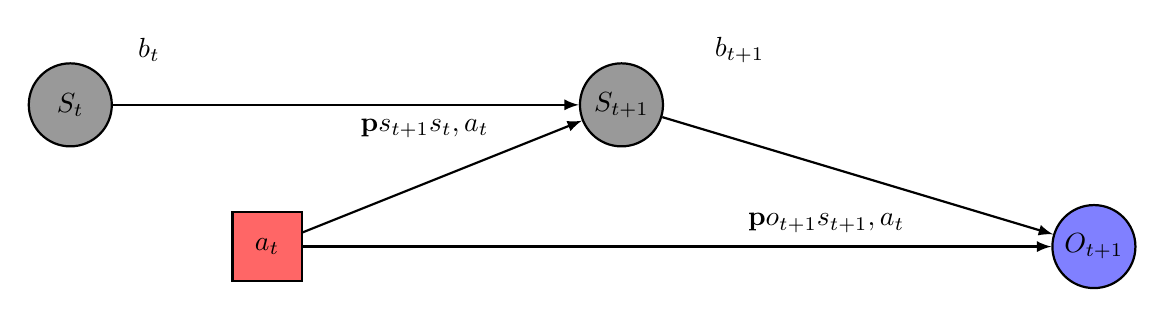
\begin{tikzpicture}
%%%%%%%%%%%%%%%%%%%%%%%%%%%%%%%%%%%%%%%%%%%%%%%%%%%%%%%%%%%%%%
%vertex
\tikzstyle{vertex}=[circle,fill=black!40,minimum size=30pt,inner sep=0pt,draw=black,thick]
\tikzstyle{avertex}=[rectangle,fill=red! 60,minimum size=25pt,inner sep=0pt,draw=black,thick]
\definecolor{darkgreen}{rgb}{0.3,0.8,0.5}
\tikzstyle{overtex}=[circle,fill=blue!50,minimum size=30pt,inner sep=0pt,draw=black,thick]
%nodes
\node[vertex] (state1) at (0,1.8) {$S_t$};
\node[vertex] (state2) at (7,1.8) {$S_{t+1}$};
\node[overtex] (obs) at (13,0) {$O_{t+1}$};
\node[avertex] (action) at (2.5,0) {$a_t$};
%%bels
\node (bel1) at (1,2.5) {$b_t$};
\node (bel2) at (8.5,2.5) {$b_{t+1}$};
%probas
\node (trans) at (4.5,1.5) {$\textbf{p} \paren{ s_{t+1} \sachant s_t, a_t }$};
\node (observ) at (9.6,0.3) {$\textbf{p} \paren{ o_{t+1} \sachant s_{t+1}, a_t }$};
%%%%%%%%%%%%%%%%%%%%%%%%%%%%%%%%%%%%%%%%%%%%%%%%%%%%%%%%%%%%%%
%ARROWS
\draw[->,>=latex, thick] (state1) -- (state2);
\draw[->,>=latex, thick] (state2) -- (obs);
\draw[->,>=latex, thick] (action) -- (state2);
\draw[->,>=latex, thick] (action) -- (obs);
\end{tikzpicture}
\caption[Bayesian Network illustrating the belief update.]{Bayesian Network illustrating the belief update: the states are the gray circular nodes, 
the action is the red square node, and the observation is the blue circular node.
The random variable $S_{t+1}$ representing the next state $s_{t+1}$ 
depends on the current one $s_t$ and on the current action $a_t$.
The random variable $O_{t+1}$ representing the next observation $o_{t+1}$ 
depends on the next state $s_{t+1}$ 
and on the current action $a_t$ too.
The belief state $b_{t}$ (resp. $b_{t+1}$)
is the probabilistic estimation of the current (resp. next) system state $s_t$ (resp. $s_{t+1}$).}
\label{BayesNetPOMDP}
\end{figure}%

As successive beliefs are computed 
with the observations perceived by the agent,
they are considered as visible by the agent. 
%Moreover, it can be easily shown that
%the expected total reward can be rewritten 
%\begin{equation}
%\label{probCriterion}
%\mathbb{E} \croch{ \sum_{t=0}^{+ \infty} \gamma^t r(s_t,d_t) } = \mathbb{E} \croch{ \sum_{t=0}^{+ \infty} \gamma^t r(b_t,d_t) }, 
%\end{equation}
%defining $r(b_t,a) = \sum_s r(s,a) \cdot b_t(s)$ as the reward of belief $b_t$.
Let us denote by $\mathbb{P}^{\mathcal{S}}$ 
the infinite set of probability distributions 
over $\mathcal{S}$.
An optimal strategy can be looked for 
as a function $d$ defined on $\mathbb{P}^{\mathcal{S}}$ 
such that successive $d_t = d(b_t) \in \mathcal{A}$ 
maximize the expected reward (\ref{criterion}):
the agent decisions are then based on the belief state.

%
% POMDP ROBOTICS
%
The POMDP framework is a flexible model for autonomous robotics,
as illustrated by the firefighter example, see Figure \ref{robot_pompier}:
it allows to describe all the robotic and surrounding system,
as well as the robot's mission,
and it is commonly used in robotics 
\cite{conf/isrr/PineauG05,OngShaoHsuWee-IJRR10,DBLP:conf/rss/Marthi12,DBLP:conf/ecai/ChanelTL12,DBLP:conf/aaai/ChanelTL13}.
It takes into account that the robot receives data
from its sensors only,
and thus has to figure out the actual system state 
using these data, named observations,
in order to fulfill the mission.
However the POMDP model raises some issues,
in particular in the robotic context.

%
% HIGH COMPLEXITY
%
\section*{Practical issues of the POMDP framework}
\subsection*{Complexity}
Solving a POMDP \textit{i.e.} computing an optimal strategy, 
is PSPACE-hard in finite horizon \cite{Papadimitriou:1987} 
and even
undecidable in infinite horizon \cite{Madani:1999:UPP:315149.315395}.
Moreover a space exponential in the problem description may be required 
for an explicit specification of such a strategy.
See \cite{Mundhenk:2000:CPP:867838} 
for a more detailed complexity analysis of POMDPs.

This high complexity is well-known by POMDP practitioners:
optimality can only be reached 
for tiny problems, 
or highly structured ones.
Classical approaches try to solve this problem
using Dynamic Programming 
and linear programming techniques \cite{Cassandra97incrementalpruning}.
Otherwise, only approximate solutions can be computed,
and thus the strategy has no optimality guaranty.
For instance, popular approaches such as point-based methods 
\cite{Pineau_2003_4826,Kurniawati-RSS08,Smith:2004:HSV:1036843.1036906}, 
grid-based ones \cite{Geffner98solvinglarge,Brafman97aheuristic,Bonet_newgrid-based}
or Monte Carlo approaches \cite{NIPS2010_4031},
use approximate computations.
The next POMDP's practical issues that will be highlighted, 
concern modeling flaws appearing when using this framework:
they are easily illustrated via robotic situations.

%
% VISION IN ROBOTICS
%
\begin{figure} \centering
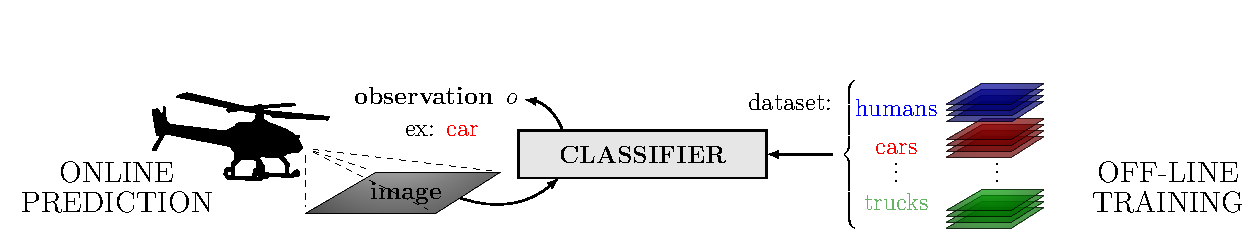
\includegraphics[scale=0.75]{fig2}
\caption[Example of an observation method in a robotic context]{
Example of an observation method in a robotic context:
the robot, here a drone, is equipped with a camera
and uses a classifier computed from a image dataset
(as NORB, see Figure \ref{NORB}): 
such a classifier is described in Figure \ref{CV_algoConvNet}.
The classifier is generated before the mission (off-line)
with a image dataset (see the right part of the illustration),
and the classifier output is used during the mission (online) 
as an observation, for the agent (see the left part).
Here, observations are thus generated by computer vision means.}
\label{observation_robot}
\end{figure}
%
% VISION IN ROBOTICS END
%


%
% COMPUTER VISION
%
\subsection*{Parameter imprecision and computer vision}
Consider now robots using visual perception, 
and whose observations 
come from computer vision algorithms based on statistical learning
(see, for instance, Figure \ref{observation_robot}).
In this situation, the robot uses a \textit{classifier}
to recognize objects in images: 
the classifier is supposed to return the name of 
the object actually in the image, 
and makes some mistakes 
with a low probability 
(see confusion matrix of Figure \ref{confusion_matrix}).

The classifier is computed using a \textit{training dataset} of images
(as NORB, see Figure \ref{NORB}, authors made it available at \url{http://www.cs.nyu.edu/~ylclab/data/norb-v1.0/}).
A powerful gradient-based learning algorithm meant to compute classifiers using image datasets
is described in Figure \ref{CV_algoConvNet}: the associated framework is called Convolutional Nextwork \cite{Lecun98gradient-basedlearning}.
Figures (\ref{NORB}), (\ref{CV_algoConvNet}) and (\ref{confusion_matrix})
illustrate the example of a classifier computed for a UAV mission where features of interests
(system states of the problem) 
are related with the presence (or absence) of animals, cars, humans, planes or trucks:
the statistical problem of computing a classifier recognizing such objects in images 
is called \textit{multiclass classification}.

%%%
%%% NORB DATA SET
%%%
\newcounter{moncompteur} %define counter
\begin{figure} \centering
\begin{tikzpicture}
\node (notes) at (1cm,7cm) { 
NORB dataset: \color{blue} $(\mbox{image}_i,\mbox{label}_i)_{i=1}^N$
};

\def\names{{"bla","human","car","truck","truck","nothing","nothing","nothing","truck"}}%
\def\namess{{"bla","airplane","car","human","animal","car","human","animal","animal"}}%

\setcounter{moncompteur}{1}
	\coordinate (norb11) at (6.2cm,3.05cm); 
	\coordinate (norb12) at (14cm,3.05cm); 
	\coordinate (norb11lab) at (6.2cm,6.2cm); 
	\coordinate (norb12lab) at (14cm,6.2cm); 
	\coordinate (norb11lab2) at (6.2cm,1.9cm); 
	\coordinate (norb12lab2) at (14cm,1.9cm); 
	\foreach \y in {0.25,0.5,...,2} {
		\coordinate (weight) at (barycentric cs:norb11= \y,norb12=1-\y);
		\def\reptemp{photos/} %define string
		\appto\reptemp{\themoncompteur} %access the string of a counter
		\appto\reptemp{.png} % concatenate two trings
		\node (image) at (weight) {\includegraphics[scale=0.5]{\reptemp}};
		
		\coordinate (weight2) at (barycentric cs:norb11lab= \y,norb12lab=1-\y);
		\node[scale=0.7] (leslabels) at (weight2) {\pgfmathparse{\names[\themoncompteur]}\pgfmathresult};
		\coordinate (weight3) at (barycentric cs:norb11lab2= \y,norb12lab2=1-\y);
		\node[scale=0.7] (leslabels) at (weight3) {\pgfmathparse{\namess[\themoncompteur]}\pgfmathresult};

		\addtocounter{moncompteur}{1}
	}

	\coordinate (norb21) at (6.2cm,5cm); 
	\coordinate (norb22) at (14cm,5cm); 
	\foreach \y in {0.25,0.5,...,2} {
		\coordinate (weight) at (barycentric cs:norb21= \y,norb22=1-\y);
		\def\reptemp{photos/} %define string
		\appto\reptemp{\themoncompteur} %access the string of a counter
		\appto\reptemp{.png} % concatenate two trings
		\node (image) at (weight) {\includegraphics[scale=0.5]{\reptemp}};
		\addtocounter{moncompteur}{1}
	}

\end{tikzpicture}
\caption[Example of image dataset for computer vision.]{Example of image dataset for computer vision: 
the labeled image dataset NORB \cite{LeCun.2004}. The size of NORB is higher than $3.10^5$,
and images from this dataset represents objects among the $5$ classes: 
``animal'', ``car'', ``human'', ``nothing'', ``plane'' and ``truck''.
Each element of a labeled image dataset is composed of a image (e.g. a image showing a car)
and a label corresponding to the class of the object represented by the image 
(in the previous example, the label is ``car'').
This dataset can be used for supervised learning to compute a classifier (see Figure \ref{CV_algoConvNet}).
In order to be able to discern locations of targets, 
a image is labeled with the name of centered object 
(``nothing'' if there is nothing in the image center).}
\label{NORB}
\end{figure}
%%%%%
%%%%% NORB DATASET END
%%%%%

%
% IMPRECISION OBSERVATION
%
As the classifier is learned based on a image dataset 
(see weights learned in Figure \ref{CV_algoConvNet}),
its behavior, and thus its performances 
(\textit{i.e.} how well it predicts objects in images) 
are inevitably dependent on the dataset.
It is a problem if the image variability in the dataset
is too low:
in this case, the probabilistic behavior of the classifier 
will be dependent on these particular images, 
and the robotic system will have poor observation
capabilities when the considered mission involves 
images too different from the ones from the dataset. 

Some large image datasets with a high image variability exists 
(e.g. NORB, Figure \ref{NORB}, although variability could be ideally higher):
note however that with such datasets, the vision performances are reduced,
or good performances are, at least, harder to reach.

A confusion matrix can be computed (see Figure \ref{confusion_matrix})
using such a labeled image dataset,
not used for the training, and called \textit{testing dataset}: 
observation frequencies can be deduced from this matrix,
normalizing rows into probabilities.
A row corresponds to an object in the scene,
and probabilities on this row are observation probabilities,
\textit{i.e.} each probability is the frequency with which 
the classifier returns the name of the object of the corresponding column.
These probabilities can be used to define the observation function 
$\textbf{p} \paren{o' \sachant s',a}$
introduced above. 
This approach raises the issue of knowing if the testing dataset 
is representative enough of the mission reality.
If not, the observation probabilities may not be reliable,
and the POMDP badly defined: 
however, as shown by the equation (\ref{probBayesRule})
the belief update needs a perfect knowledge of the
observation probability distributions.

More generally, observations of the agent 
may be outputs of image processing algorithms 
whose semantics (image correlation, object matching, class inference, 
preprocessing followed by classifiers such as the one computed 
in Figure \ref{CV_algoConvNet} etc.) 
are so complex that probabilities of 
occurrence are hard to rigorously extract.

Finally, if the considered datasets are labeled more precisely 
(as NORB, which includes information such as the lighting condition, or the object scale),
we can imagine that the computed observation probabilities (from the confusion matrix) 
were more reliable, or the vision performances upgraded 
(since separation when learning the classifier is easier).
However, as more observation or states are involved in this case,
the POMDP is harder to solve.
Moreover, as the number of images per class is reduced 
(since there are more complex and numerous classes), 
a poorer confusion matrix is obtained when testing (in terms of confidence).

As a conclusion, the POMDP model supposes 
the knowledge of all
probability distributions involved:
unfortunately the actual frequencies 
used to compute them
are not precisely known in practice.
The imprecision about these probabilities, 
for instance the imprecision related to 
the vision algorithm behavior
with real world images,
has to be taken into account 
to make the robot autonomous 
under any circumstances.
In general, the computation 
of the probability distributions
of a POMDP needs enough tests 
for each possible system state and action,
which is hard to perform:
there are limited data to learn the model
in practice.

%%
%% ConvNets
%%
\begin{figure} \centering
\begin{tikzpicture} 
\label{bipyr}
%%%%%%%%%%%%%%%%%%%%%%%%%%%%%%%%%%%%%%%%%%%%%%%%%%%%%%%%%%%%%%%%%%%%%%%%%%%%%%% TIKZ
%%%%%%%%%%%%%%%%%%%%%%%%%%%%%%%%%%%%%%%%%%%%%%%%%%%%%%%%%%%%%%%%%%%%%%%%%%%%%%%

\node (car) at (-1,-1) {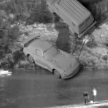
\includegraphics[scale=0.52]{NORB_car.png}};

	% input image 
	\coordinate (A1) at (0cm,0cm); 
	\coordinate (A2) at (0cm,-2cm); 
	\coordinate (A3) at (-2cm,0cm);
	\coordinate (A4) at (-2cm,-2cm); 
	\draw[thick] (A1) -- (A3);
	\draw[thick] (A3) -- (A4);
	\draw[thick] (A4) -- (A2);
	\draw[thick] (A2) -- (A4);

	\node at (barycentric cs:A1=1,A3=1,A2=-0.15) {\tiny $m$};
	\node at (barycentric cs:A3=1,A4=1,A1=-0.2) {\tiny $m$};

	% output feature
	\coordinate (A6) at (7cm,-4cm);
	\coordinate (A7) at (9cm,-0.7cm);
	\coordinate (A8) at (9.1cm,-0.7cm);
	\coordinate (A9) at (7.1cm,-4cm);
	\draw[thick] (A6) -- (A9);
	\draw[thick] (A7) -- (A8);
	\draw[thick] (A8) -- (A9);

	\node at (barycentric cs:A7=1,A8=1,A6=-0.1) {\tiny $1$};
	\node at (barycentric cs:A8=1,A9=1,A1=-0.05) {\tiny $n$};

	%% draw faces
	%\fill[gray!50,opacity=0.7] (A1) -- (A6) -- (A7) -- cycle;
	%\fill[gray!50,opacity=0] (A1) -- (A2) -- (A7) -- cycle; 
	%\fill[gray!50,opacity=0.7] (A2) -- (A1) -- (A6) -- cycle;
	\draw[thick,dashed] (A1) -- (A7);
	\draw[thick,dashed] (A2) -- (A7);

	%%%%%%%%%%%%%%%%%%%%%%%%%%%%%%%%%%%%%%%
	%% INTERMEDIATE FEATURE MAPS DRAWING %%
	%%%%%%%%%%%%%%%%%%%%%%%%%%%%%%%%%%%%%%%

	%%%%%%%%%%%%%%%%%%%%%%%%%%%%%%%%%%%%%%%%%%%%%%%%%%%%%%% LINE1

	% base points (of right and left images)
	\coordinate (im111) at (2.77cm,-0.08cm); 
	\coordinate (im112) at (2.77cm,-1.85cm); 
	\coordinate (im113) at (1cm,-0.08cm);
	\coordinate (im114) at (1cm,-1.85cm); 

	\coordinate (im131) at (2.45cm,-0.4cm); 
	\coordinate (im132) at (2.45cm,-2.17cm); 
	\coordinate (im133) at (0.68cm,-0.4cm);
	\coordinate (im134) at (0.68cm,-2.17cm); 


	% images plans
	% beginning
	\draw[thick] (im111) -- (im113);
	\draw[thick] (im113) -- (im114);
	\draw[thick] (im114) -- (im112);
	\draw[thick] (im112) -- (im111);
	\fill[gray!00,opacity=0.7] (im111) -- (im112) -- (im114) -- (im113) -- cycle;


	% intermediate plans
	\coordinate (im121) at (2.62cm,-0.24cm); 
	\coordinate (im122) at (2.62cm,-2.01cm); 
	\coordinate (im123) at (0.85cm,-0.24cm);
	\coordinate (im124) at (0.85cm,-2.01cm); 
	\draw[thick] (im121) -- (im123);
	\draw[thick] (im123) -- (im124);
	\draw[thick] (im124) -- (im122);
	\draw[thick] (im122) -- (im121);
	\fill[gray!00,opacity=0.7] (im121) -- (im122) -- (im124) -- (im123) -- cycle;

	%% end
	\draw[thick] (im131) -- (im133);
	\draw[thick] (im133) -- (im134);
	\draw[thick] (im134) -- (im132);
	\draw[thick] (im132) -- (im131);
	\fill[gray!00,opacity=0.7] (im131) -- (im132) -- (im134) -- (im133) -- cycle;


	%%%%%%%%%%%%%%%%%%%%%%%%%%%%%%%%%%%%%%%%%%%%%%%%%%%%%%% LINE2
	
	% base points (of right and left images)
	\coordinate (im211) at (4.5cm,-2cm); 
	\coordinate (im212) at (4.5cm,-3cm); 
	\coordinate (im213) at (3.5cm,-2cm);
	\coordinate (im214) at (3.5cm,-3cm); 

	\coordinate (im291) at (5.5cm,-0.35cm); 
	\coordinate (im292) at (5.5cm,-1.35cm); 
	\coordinate (im293) at (4.5cm,-0.35cm);
	\coordinate (im294) at (4.5cm,-1.35cm); 

	% images plans
	% beginning
	\draw[thick] (im291) -- (im293);
	\draw[thick] (im293) -- (im294);
	\draw[thick] (im294) -- (im292);
	\draw[thick] (im292) -- (im291);
	\fill[gray!00,opacity=0.7] (im291) -- (im292) -- (im294) -- (im293) -- cycle;

	% intermediate plans
	\foreach \y in {0.1,0.2,...,1} {
		\coordinate (ii1) at (barycentric cs:im211= \y,im291=1-\y);
		\coordinate (ii2) at (barycentric cs:im212= \y,im292=1-\y);
		\coordinate (ii3) at (barycentric cs:im213= \y,im293=1-\y);
		\coordinate (ii4) at (barycentric cs:im214= \y,im294=1-\y);

		\draw[thick] (ii1) -- (ii3);
		\draw[thick] (ii3) -- (ii4);
		\draw[thick] (ii4) -- (ii2);
		\draw[thick] (ii2) -- (ii1);
		\fill[gray!00,opacity=0.7] (ii1) -- (ii2) -- (ii4) -- (ii3) -- cycle;
	}

	% end
	\draw[thick] (im211) -- (im213);
	\draw[thick] (im213) -- (im214);
	\draw[thick] (im214) -- (im212);
	\draw[thick] (im212) -- (im211);
	\fill[gray!00,opacity=0.7] (im211) -- (im212) -- (im214) -- (im213) -- cycle;

	%%%%%%%%%%%%%%%%%%%%%%%%%%%%%%%%%%%%%%%%%%%%%%%%%%%%%%% LINE3

	% base points (of right and left images)
	\coordinate (im311) at (5.75cm,-3cm); 
	\coordinate (im312) at (5.75cm,-3.5cm); 
	\coordinate (im313) at (5.25cm,-3cm);
	\coordinate (im314) at (5.25cm,-3.5cm); 

	\coordinate (im391) at (7.2cm,-0.53cm); 
	\coordinate (im392) at (7.2cm,-1.03cm); 
	\coordinate (im393) at (6.7cm,-0.53cm);
	\coordinate (im394) at (6.7cm,-1.03cm); 

	% images plans
	% beginning
	\draw[thick] (im391) -- (im393);
	\draw[thick] (im393) -- (im394);
	\draw[thick] (im394) -- (im392);
	\draw[thick] (im392) -- (im391);
	\fill[gray!00,opacity=0.7] (im391) -- (im392) -- (im394) -- (im393) -- cycle;

	% intermediate plans
	\foreach \y in {0.05,0.1,...,1} {
		\coordinate (ii1) at (barycentric cs:im311= \y,im391=1-\y);
		\coordinate (ii2) at (barycentric cs:im312= \y,im392=1-\y);
		\coordinate (ii3) at (barycentric cs:im313= \y,im393=1-\y);
		\coordinate (ii4) at (barycentric cs:im314= \y,im394=1-\y);

		\draw[thick] (ii1) -- (ii3);
		\draw[thick] (ii3) -- (ii4);
		\draw[thick] (ii4) -- (ii2);
		\draw[thick] (ii2) -- (ii1);
		\fill[gray!00,opacity=0.7] (ii1) -- (ii2) -- (ii4) -- (ii3) -- cycle;
	}

	% end
	\draw[thick] (im311) -- (im313);
	\draw[thick] (im313) -- (im314);
	\draw[thick] (im314) -- (im312);
	\draw[thick] (im312) -- (im311);
	\fill[gray!00,opacity=0.7] (im311) -- (im312) -- (im314) -- (im313) -- cycle;

	%%%%%%%%%%%%%%%%%%%%%%%%%%%%%%%%%%%%%%%%%%%%%%%%%%%%%%% LINE4
	
	% base points (of right and left images)
	\coordinate (im411) at (6.35cm,-3.5cm); 
	\coordinate (im412) at (6.35cm,-3.75cm); 
	\coordinate (im413) at (6.1cm,-3.5cm);
	\coordinate (im414) at (6.1cm,-3.75cm); 

	\coordinate (im491) at (8.12cm,-0.61cm); 
	\coordinate (im492) at (8.12cm,-0.86cm); 
	\coordinate (im493) at (7.87cm,-0.61cm);
	\coordinate (im494) at (7.87cm,-0.86cm); 

	% images plans
	% beginning
	\draw[thick] (im491) -- (im493);
	\draw[thick] (im493) -- (im494);
	\draw[thick] (im494) -- (im492);
	\draw[thick] (im492) -- (im491);
	\fill[gray!00,opacity=0.8] (im491) -- (im492) -- (im494) -- (im493) -- cycle;

	% intermediate plans
	\foreach \y in {0.04,0.08,...,1} {
		\coordinate (ii1) at (barycentric cs:im411= \y,im491=1-\y);
		\coordinate (ii2) at (barycentric cs:im412= \y,im492=1-\y);
		\coordinate (ii3) at (barycentric cs:im413= \y,im493=1-\y);
		\coordinate (ii4) at (barycentric cs:im414= \y,im494=1-\y);

		\draw[thick] (ii1) -- (ii3);
		\draw[thick] (ii3) -- (ii4);
		\draw[thick] (ii4) -- (ii2);
		\draw[thick] (ii2) -- (ii1);
		\fill[gray!00,opacity=0.7] (ii1) -- (ii2) -- (ii4) -- (ii3) -- cycle;
	}

	% end
	\draw[thick] (im411) -- (im413);
	\draw[thick] (im413) -- (im414);
	\draw[thick] (im414) -- (im412);
	\draw[thick] (im412) -- (im411);
	\fill[gray!00,opacity=0.8] (im411) -- (im412) -- (im414) -- (im413) -- cycle;


	%%%%%%%%%%%%%%%%%%%%%%%%%%%%%%%%%%%%%%%%%%%%%%%%%%%%%%% LINE5

	% base points (of right and left images)
	\coordinate (im511) at (6.75cm,-3.8cm); 
	\coordinate (im512) at (6.75cm,-3.9cm); 
	\coordinate (im513) at (6.65cm,-3.8cm);
	\coordinate (im514) at (6.65cm,-3.9cm); 

	\coordinate (im591) at (8.65cm,-0.67cm); 
	\coordinate (im592) at (8.65cm,-0.77cm); 
	\coordinate (im593) at (8.55cm,-0.67cm);
	\coordinate (im594) at (8.55cm,-0.77cm); 

	% images plans
	% beginning
	\draw[thick] (im591) -- (im593);
	\draw[thick] (im593) -- (im594);
	\draw[thick] (im594) -- (im592);
	\draw[thick] (im592) -- (im591);
	\fill[gray!00,opacity=0.8] (im591) -- (im592) -- (im594) -- (im593) -- cycle;

	% intermediate plans
	\foreach \y in {0.025,0.05,...,1} {
		\coordinate (ii1) at (barycentric cs:im511= \y,im591=1-\y);
		\coordinate (ii2) at (barycentric cs:im512= \y,im592=1-\y);
		\coordinate (ii3) at (barycentric cs:im513= \y,im593=1-\y);
		\coordinate (ii4) at (barycentric cs:im514= \y,im594=1-\y);

		\draw[thick] (ii1) -- (ii3);
		\draw[thick] (ii3) -- (ii4);
		\draw[thick] (ii4) -- (ii2);
		\draw[thick] (ii2) -- (ii1);
		\fill[gray!00,opacity=0.7] (ii1) -- (ii2) -- (ii4) -- (ii3) -- cycle;
	}

	% end
	\draw[thick] (im511) -- (im513);
	\draw[thick] (im513) -- (im514);
	\draw[thick] (im514) -- (im512);
	\draw[thick] (im512) -- (im511);
	\fill[gray!00,opacity=0.8] (im511) -- (im512) -- (im514) -- (im513) -- cycle;


	%%%%%%%%%%%%%%%%%%%%%%	
	%% END FEATURE MAPS %%
	%%%%%%%%%%%%%%%%%%%%%%

	\draw[thick,dashed] (A2) -- (A6);
	\draw[thick] (A7) -- (A6);
	\draw[thick,dashed] (A1) -- (A6);
	\draw[thick] (A1) -- (A2);
	
	% draw points
	\foreach \i in {1,2,3,4,6,7,8,9}
	{
	  \draw[fill=black] (A\i) circle (0.01em);
	}

	% draw arrows
	\coordinate (F1) at (-0.5,-2.2cm);
	\coordinate (F2) at (0.7,-2.5cm);
	\coordinate (F3) at (1.7,-2.8cm);
	\coordinate (F4) at (3.2,-3.1cm);
	\coordinate (F5) at (4,-3.4cm);
	\coordinate (F6) at (5,-3.7cm);
	\node (Fdots) at (5.6,-3.9cm) [rotate=345] {$\ldots$};
	\coordinate (F7) at (6.6,-4.05cm);
	\coordinate (F8) at (7,-4.1cm);
	\coordinate (F9) at (7.3,-4.1cm);
	\coordinate (F10) at (8.7,-3.2cm);

	\draw[->,>=latex,thick, color=blue!60] (F1) to[bend right] (F2);
	\draw[->,>=latex,thick, color=blue!60] (F3) to[bend right] (F4);
	\draw[->,>=latex,thick, color=blue!60] (F5) to[bend right] (F6);
	\draw[->,>=latex,thick, color=blue!60] (F7) to[bend right] (F8);
	\draw[->,>=latex,thick, color=blue!60] (F9) to[bend right] (F10);

	\coordinate (A10) at (8.7cm,-3cm);
	\coordinate (A11) at (9.55cm,-1.7cm);
	\coordinate (A12) at (9.65cm,-1.7cm);
	\coordinate (A13) at (8.8cm,-3cm);
	\draw[thick] (A10) -- (A11);
	\draw[thick] (A11) -- (A12);
	\draw[thick] (A12) -- (A13);
	\draw[thick] (A13) -- (A10);
%%%%%%%%%%%%%%%%%%%%%%%%%%%%%%%%%%%%%%%%%%%%%%%%%%%%%%%%%%%%%%%%%%
%%%%%%%%%%%%%%%%%%%%%%%%%%%%%%%%%%%%%%%%%%%%%%%%%%%%%%%%%%%%%%%%%%
%****************************************************************%
%%%%%%%%%%%%%%%%%%%%%%%%%%%%%%%%%%%%%%%%%%%%%%%%%%%%%%%%%%%%%%%%%%
%%%%%%%%%%%%%%%%%%%%%%%%%%%%%%%%%%%%%%%%%%%%%%%%%%%%%%%%%%%%%%%%%%

	\node at (-0.3,0.8) {Given $i \in \set{1,\ldots,N}$,};
	\node at (barycentric cs:A2=1,A4=1,A1=-0.4) {\color{blue} $\mbox{picture}_i$};


	\draw[thick,dashed] (A9) -- (A10);
	\draw[thick,dashed] (A8) -- (A11);
	\node (etiq2) at (barycentric cs:A12=1,A13=1,A1=-0.2) {$\mbox{vector}_{\color{black}i}^{\color{red}W}$};

	\node (w0) at (0.3cm, -3cm) {{\color{red} $w_0$ }};
	\node (w1) at (2.2cm, -3.5cm) {{\color{red} $w_1$ }};
	\node (w2) at (4cm, -3.9cm) {{\color{red} $w_2$ }};
	\node (wm) at (9cm, -4cm) {{\color{red} $w_m$ }};

	\node  at (12cm,0cm) {\color{blue} $\mbox{label}_i$};
	\node (etiq) at (12cm,-0.7cm) {e.g. ``car''};


\tikzstyle{grisEncadre}=[thick, fill=gray!20];
\draw [grisEncadre] (6.8,-4.65) rectangle (13.2,-5.9);

	\node (perte) at (11.3cm, -4.7cm) {};	
	\node (perte1) at (10cm, -4.9cm) { \textit{gradient-based} \textit{ minimization} of};
	\node (perte2) at (10cm, -5.5cm) {  $loss\Big( (\mbox{vector}_{\color{black}i}^{\color{red}W})_{i=1}^N, ({\color{blue} \mbox{label}_i})_{i=1}^N \Big)$ in {\color{red} W}};
	

	\draw[->,>=latex,thick, color=blue!60,line width=1mm] (etiq) to (perte);
	\draw[->,>=latex,thick, color=blue!60,line width=1mm] (etiq2) to (perte);
	

	\node (Wpictures) at (-0.1cm,-4cm) {{\color{red} $W$:}};

	\node (Wpictures2) at (2.55cm,-4.5cm) {};
	\node (classifieur) at (1.1cm,-4.5cm) {};

	\node (perte3) at (6.92cm, -5.2cm) {};

	\node (lesweights) at (5cm, -5.4cm) { { \color{red} $\left . \begin{array}{ccccc}
	\\
	\\
	\\
	\\
	\\
	\end{array} \right \}$}};
	\node (w) at (5.4cm, -5.2cm) {};
	\draw[->,>=latex,thick, color=red!60, line width=1mm] (perte3) to (w);

% to rename files in a directory in a correct way:
% compteur=0
% for file in *.png; do compteur=$((compteur+1)); echo $compteur; mv $file $compteur.png; done
%%%% WARNING!!! IT REMOVE SOME FILES!


	\setcounter{moncompteur}{171}

	\coordinate (ligne01) at (0cm,-4.4cm); 
	\coordinate (ligne02) at (5cm,-4.4cm); 
	\foreach \y in {0.05,0.1,...,1} {
		\coordinate (weight) at (barycentric cs:ligne01= \y,ligne02=1-\y);
		\def\reptemp{weights/} %define string
		\appto\reptemp{\themoncompteur} %access the string of a counter
		\appto\reptemp{.png} % concatenate two trings
		\node (image) at (weight) {\includegraphics{\reptemp}};
		\addtocounter{moncompteur}{1}
	}	


	\coordinate (ligne11) at (0cm,-4.65cm); 
	\coordinate (ligne12) at (5cm,-4.65cm); 
	\foreach \y in {0.05,0.1,...,1} {
		\coordinate (weight) at (barycentric cs:ligne11= \y,ligne12=1-\y);
		\def\reptemp{weights/} %define string
		\appto\reptemp{\themoncompteur} %access the string of a counter
		\appto\reptemp{.png} % concatenate two trings
		\node (image) at (weight) {\includegraphics{\reptemp}};
		\addtocounter{moncompteur}{1}
	}

	
	\coordinate (ligne21) at (0cm,-4.9cm); 
	\coordinate (ligne22) at (5cm,-4.9cm); 
	\foreach \y in {0.05,0.1,...,1} {
		\coordinate (weight) at (barycentric cs:ligne21= \y,ligne22=1-\y);
		\def\reptemp{weights/} %define string
		\appto\reptemp{\themoncompteur} %access the string of a counter
		\appto\reptemp{.png} % concatenate two trings
		\node (image) at (weight) {\includegraphics{\reptemp}};
		\addtocounter{moncompteur}{1}
	}

	\coordinate (ligne31) at (0cm,-5.15cm); 
	\coordinate (ligne32) at (5cm,-5.15cm); 
	\foreach \y in {0.05,0.1,...,1} {
		\coordinate (weight) at (barycentric cs:ligne31= \y,ligne32=1-\y);
		\def\reptemp{weights/} %define string
		\appto\reptemp{\themoncompteur} %access the string of a counter
		\appto\reptemp{.png} % concatenate two trings
		\node (image) at (weight) {\includegraphics{\reptemp}};
		\addtocounter{moncompteur}{1}
	}

	\coordinate (ligne41) at (0cm,-5.4cm); 
	\coordinate (ligne42) at (5cm,-5.4cm); 
	\foreach \y in {0.05,0.1,...,1} {
		\coordinate (weight) at (barycentric cs:ligne41= \y,ligne42=1-\y);
		\def\reptemp{weights/} %define string
		\appto\reptemp{\themoncompteur} %access the string of a counter
		\appto\reptemp{.png} % concatenate two trings
		\node (image) at (weight) {\includegraphics{\reptemp}};
		\addtocounter{moncompteur}{1}
	}

	\coordinate (ligne51) at (0cm,-5.65cm); 
	\coordinate (ligne52) at (5cm,-5.65cm); 
	\foreach \y in {0.05,0.1,...,1} {
		\coordinate (weight) at (barycentric cs:ligne51= \y,ligne52=1-\y);
		\def\reptemp{weights/} %define string
		\appto\reptemp{\themoncompteur} %access the string of a counter
		\appto\reptemp{.png} % concatenate two trings
		\node (image) at (weight) {\includegraphics{\reptemp}};
		\addtocounter{moncompteur}{1}
	}

	\coordinate (ligne61) at (0cm,-5.9cm); 
	\coordinate (ligne62) at (5cm,-5.9cm); 
	\foreach \y in {0.05,0.1,...,1} {
		\coordinate (weight) at (barycentric cs:ligne61= \y,ligne62=1-\y);
		\def\reptemp{weights/} %define string
		\appto\reptemp{\themoncompteur} %access the string of a counter
		\appto\reptemp{.png} % concatenate two trings
		\node (image) at (weight) {\includegraphics{\reptemp}};
		\addtocounter{moncompteur}{1}
	}

	\coordinate (ligne71) at (0cm,-6.15cm); 
	\coordinate (ligne72) at (5cm,-6.15cm); 
	\foreach \y in {0.05,0.1,...,1} {
		\coordinate (weight) at (barycentric cs:ligne71= \y,ligne72=1-\y);
		\def\reptemp{weights/} %define string
		\appto\reptemp{\themoncompteur} %access the string of a counter
		\appto\reptemp{.png} % concatenate two trings
		\node (image) at (weight) {\includegraphics{\reptemp}};
		\addtocounter{moncompteur}{1}
	}

	\coordinate (ligne81) at (0cm,-6.4cm); 
	\coordinate (ligne82) at (5cm,-6.4cm); 
	\foreach \y in {0.05,0.1,...,1} {
		\coordinate (weight) at (barycentric cs:ligne81= \y,ligne82=1-\y);
		\def\reptemp{weights/} %define string
		\appto\reptemp{\themoncompteur} %access the string of a counter
		\appto\reptemp{.png} % concatenate two trings
		\node (image) at (weight) {\includegraphics{\reptemp}};
		\addtocounter{moncompteur}{1}
	}
\end{tikzpicture}
\caption[Example of classifier training for computer vision]{Example of classifier training for computer vision:
the labeled image dataset NORB, see Figure \ref{NORB},
is used to train and test a classifier.
The learning algorithm is based on Convolutional Network \cite{Lecun98gradient-basedlearning,DBLP:journals/jfr/SermanetHSGBECML09}
using gradient methods \cite{bottou-91c,lecun-98x,bottou-tricks-2012}.
The weights $W=(w_0,\ldots,w_m)$ are the parameters of a particular transformation 
(see the ``bi-pyramid'' of successive transformation stages) 
from the image to a vector representing a label among $\set{animal,car,human,nothing,plane,truck}$. 
These weights are learned in order to minimize a given loss function
\textit{i.e.} a proper criterion representing the error of the classifier over the dataset.
A classical loss function is the Mean Squared Error (MSE). 
The environment Torch7 (based on lua and C languages, \cite{Collobert_NIPSWORKSHOP_2011})
has been used to compute the displayed weights.
 }
\label{CV_algoConvNet}
\end{figure}
%%
%% CONVNETS END
%%

\begin{figure}[b!] \centering
\begin{tabular}{c|c|c|c|c|c!{\vrule width 2pt}c!{\vrule width 2pt}c}%!{\vrule width 2pt}}
animal & human & plane & truck & car & nothing \\ \specialrule{.2em}{.0em}{.0em}  
$3688$ & $575$ & $256$ & $48$ & $144$ & $149$ &   animal & $75.885\%$ \\ \specialrule{.05em}{.0em}{.0em}  
$97$ & $4180$ & $81$ & $20$ & $225$ & $257$ & human & $86.008\%$ \\  \specialrule{.05em}{.0em}{.0em}  
$292$ & $136$ & $3906$ & $237$ & $202$ & $87$ & plane & $80.370\%$ \\  \specialrule{.05em}{.0em}{.0em}  
$95$ & $1$ & $44$ & $4073$ & $514$ & $133$ & truck & $83.807\%$  \\  \specialrule{.05em}{.0em}{.0em}  
$129$ & $3$ & $130$ & $1283$ & $3283$ & $32$ &  car & $67.551\%$ \\  \specialrule{.05em}{.0em}{.0em}  
$154$ & $283$ & $36$ & $63$ & $61$ & $4263$ & nothing & $87.716\%$  \\ %\specialrule{.2em}{.0em}{.0em}  
\end{tabular}
\caption[Example of confusion Matrix for multiclass classification]{
Example of confusion matrix for multiclass classification:
this matrix is computed with a testing dataset of images, different from the training dataset.
Each row only considers the images of a given object,
and numbers represents the answers of the classifier: 
for instance, $3688$ images of animals are well recognized, 
but $575$ are confused with a human.
Average row correct is here $80.223\%$.
Torch7 environment \cite{Collobert_NIPSWORKSHOP_2011} has also been used 
to compute this matrix from the classifier and the testing dataset.}
\label{confusion_matrix}
\end{figure}


%
% IMPRECISION POMDP WORKS
%
Some variations of the POMDP framework 
have been built in order to take into account 
the imprecision about the probability distributions of the model, 
also called \textit{parameter imprecision}.
\subsubsection{Works handling parameter imprecision}
Here, transition and observation functions,
namely $\textbf{p} \paren{ s' \sachant s,a }$ 
and $\textbf{p} \paren{ o' \sachant s',a }$,
$\forall (s,s',o',a) \in \mathcal{S}^2 \times \mathcal{O} \times \mathcal{A}$,
are called \textit{POMDP parameters}, or yet \textit{model parameters}. 
To the best of our knowledge,
the first model meant to handle parameter imprecision
has been called POMDPIP, 
for \textit{POMDP with Imprecise Parameters} (POMDPIP) \cite{Itoh2007453}. 
In this work, each POMDP parameter is replaced by 
a set of possible parameters.
Figure \ref{uncertainty_theories}
introduces the Imprecise Probability Theory 
that inspired this idea:
in this theory, uncertainty and knowledge about it 
are represented by sets of probability distributions
(called \textit{credal sets})
to express the fact that the model is not fully known.
Imprecision of the POMDP model is well expressed in this way:
for instance, if confidence bounds on the computed probabilities
are available, 
these bounds can be taken 
into account when modeling,
considering the sets of all likely 
probability distributions.

Starting from this modeling, 
a \textit{second order belief}
is introduced in this work:
it is defined as a probability distribution 
over the possible model parameters.
This approach thus confuses
parameter imprecision and event frequency.
Indeed, strategies which are looked for
are the optimal strategies
of a particular ``averaged POMDP'': 
this POMDP results from the computation of
the average of the possible parameters 
with respect to the given second order belief.
However, the parameters of this new POMDP 
are potentially not even part of the set 
of the possible parameters.
Although POMDPIPs are well designed, 
imprecision is not really handled when 
the problem is solved
because of the use of a second order belief.
Moreover, it is claimed that the actual second order belief 
is not known, and then is allowed to vary in order to make 
the computation of an approximated strategy easier:
the analysis of performances only details 
how far is the approximated strategy 
from the ``averaged POMDP''.	

Another work, called \textit{Bounded Parameters POMDPs} 
(BPPOMDP) \cite{NiYaLiaZhi} 
does not introduce any second order belief. 
However, solving BPPOMDPs is similar 
to \cite{Itoh2007453} in spirit
since the flexibility provided by the parameter imprecision
is used to make the computations as easy as possible.
In this framework, the criterion defining optimal strategies 
is not even made explicit.

The major issue with these frameworks 
(namely POMDPIP and BPPOMDP)
is that no appropriate criterion choice is made
to manage parameter imprecision:
for instance, a suitable approach is 
to compute a cautious strategy 
regarding the imprecision \textit{i.e.} 
taking into account the worst case.
Yet, the opposite approach is to look 
for an optimistic strategy, 
considering the best case.

A more recent approach deals 
with the cautious point of view,
and is thus called 
\textit{robust POMDP} \cite{DBLP:conf/icml/Osogami15}.
Inspired by the corresponding work 
in the fully observable case 
(called \textit{uncertain MDP} \cite{NE:05}),
this work uses the well-known \textit{maximin},
or \textit{worst case} criterion,
which comes from \textit{Game Theory}: 
in this framework, an optimal strategy 
maximizes the lowest criterion
among all the parameters considered possible.
If the parameter imprecision is not stationary,
\textit{i.e.} can change at each time step,
the corresponding optimal strategy (in the maximin sense)
can be easily computed using classical computations
(called \textit{Dynamic Programming}, 
see Section \ref{subsectionDP} of Chapter \ref{chap_SOTA}).
However, when the parameter imprecision is stationary,
things become harder:
the proposed computations lead to an approximately optimal strategy,
as the handled criterion is a lower bound
of the desired maximin criterion. 
Yet, the stationary assumption for the parameter imprecision seems more suitable 
according to the proposed POMDP definition:
indeed, transition and observation functions are here defined 
as independent from the time step,
mostly to make the use of 
infinite horizon criteria 
such as (\ref{criterion}) easier.

Although the use of sets of probability distributions 
(credal sets) makes the model more consistent 
with the reality of the problem (parameters are imprecise in practice),
taking them (really) into account (e.g. with a maximin criterion) 
increases eventually the complexity 
of the optimal strategy computation.
This intuition is illustrated by Figure \ref{uncertainty_theories}:
Imprecise Probability Theory has the greatest expressiveness 
compared to the other theories,
that is why computations with this modeling 
can be expected to be harder to perform.
As explained above, POMDP solving is already a really hard task,
thus using a framework leading to more complex computations
does not seem to be a good approach. 
Moreover, with this framework, 
some restrictive assumptions are commonly needed
such as the convexity of credal sets,
and optimization may require linear programs \cite{NE:05,DBLP:conf/icml/Osogami15}.
%As discussed during this thesis 
%(for instance see Section \ref{section_expe_PPUDD} of Chapter \ref{chap_symb}),
Modeling a problem in an expressive manner may lead
to the use of important approximations without control of the latter,
as done with the POMDPIP and BPPOMDP frameworks.
It may be a better approach to start with a simpler model
which can be solved more easily in practice. 

Finally, while there are fascinating questions of algorithms in this area,
this thesis does not deal with Reinforcement Learning (RL, \cite{NIPS2009_3780,Ross:2011:BAL:1953048.2021055}), 
as we are interested in robotic applications 
whose very first executions have to proceed efficiently.
The basic reason is that robotic systems may be expensive,
and executions are not allowed to break the robot.
%The problem of interest here 
%is called \textit{offline POMDP solving}.
However, they are complementary studies:
instead of making the strategy 
as optimal as possible, 
RL improves sequentially the latter
using all the previous executions.
%for statistical learning.

\begin{figure} \centering
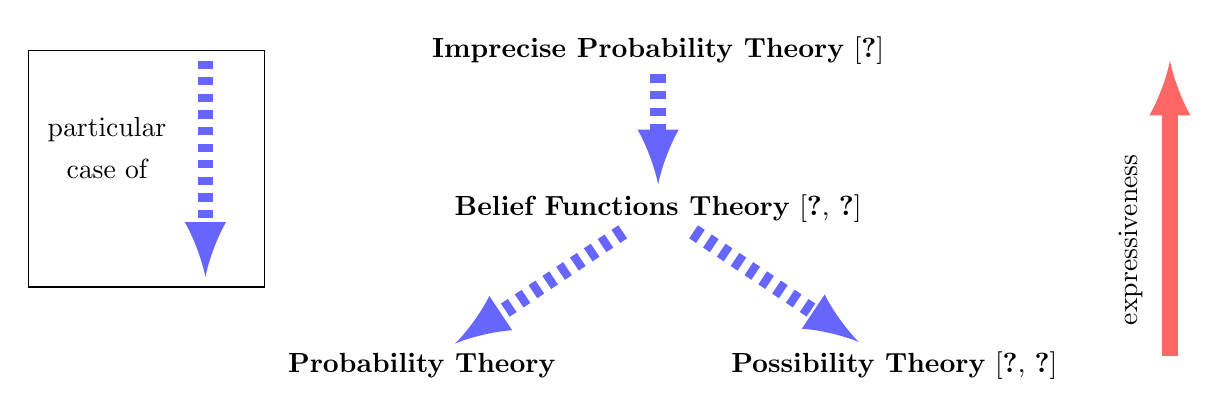
\begin{tikzpicture}
\node (IP) at (2,10) {\textbf{Imprecise Probability Theory} \cite{Walley2000125}};
\node (BF) at (2,8) {\textbf{Belief Functions Theory} \cite{dempster1967,shafer1976mathematical}};
\node (PROB) at (-1,6) {\textbf{Probability Theory}};
\node (POSS) at (5,6) {\textbf{Possibility Theory} \cite{Du2006.7,Dubois1997359}};
\draw[->,>=latex,thick, color=blue!60, line width=2mm, dashed] (IP) to (BF);
\draw[->,>=latex,thick, color=blue!60, line width=2mm, dashed] (BF) to (PROB);
\draw[->,>=latex,thick, color=blue!60, line width=2mm, dashed] (BF) to (POSS);

\node (topr) at (8.5,10) {};
\node (botr) at (8.5,6) {};
\node (middr) at (8,7.6) [rotate=90] {expressiveness};
\draw[->,>=latex,thick, color=red!60, line width=2mm] (botr) to (topr);
\draw (-6,7) rectangle (-3,10);
\node (toplegend) at (-3.75,10) {};
\node (botlegend) at (-3.75,7) {};
\draw[->,>=latex,thick, color=blue!60, line width=2mm, dashed] (toplegend) to (botlegend);
\node (bluelegend) at (-5,9) {particular};
\node (bluelegend) at (-5,8.5) {case of};
\end{tikzpicture}
\caption[Most known uncertainty theories and their relations]{Most known uncertainty theories and their relations. 
Imprecise Probability Theory (IPT) 
considers sets of probability measures
defined on the universe $\Omega$ 
in order to represent uncertainty of events 
and knowledge about it: 
this theory is the most general one. 
The Belief Functions Theory 
(BFT, or Dempster-Shafer Theory, or yet Theory of Evidence),
which is a particular case of IPT, 
considers a mass function $m$ 
defined on all the subsets of the universe,
and which sums to $1$. 
From this mass function,
upper and lower bounds
on possible probability measures
can be defined. 
The upper bound is called
plausibility measure: $\forall A \subset \Omega$, 
$Pl(A) = \sum_{B \cap A \neq \emptyset} m(B)$.
The lower bound is called the belief function:
$\forall A \subset \Omega$, 
$bel(A) = \sum_{B \subseteq A} m(B)$.
The set of probability distributions
represented by $m$ 
are all probability measures $\mathbb{P}$
such that $\forall A \subset \Omega$,
$bel(A) \leqslant \mathbb{P}(A) \leqslant Pl(A)$.
For instance, 
if the function $m$ returns $1$ for the universe,
and $0$ for all other subsets, 
it expresses the total ignorance 
about the actual probability distribution:
it corresponds to the set of all the possible 
probability distributions in IPT.
If the mass function is equal to zero 
for each non-singleton subsets,
it corresponds simply to a probability distribution
since $bel=Pl$.
If the mass function is positive only on a
sequence of nested subsets, 
it corresponds to a possibility distribution:
$bel$ is then called the \textbf{necessity measure},
and $Pl$ the \textbf{possibility measure} (see Section \ref{posspres} of Chapter \ref{chap_SOTA}).
Probability and Possibility Theory are thus
particular cases of BFT and a fortiori of IPT.}
\label{uncertainty_theories}
\end{figure}

Another practical issue of the POMDP model
may be also pointed out: 
it is about the definition of
the belief state concerning the very first
state of the system,
and more generally about
how agent knowledge is represented.
%%
%%  FULL IGNORANCE/ KNOWLEDGE OF THE AGENT
%%
\subsection*{Agent ignorance modeling}
The initial belief state $b_0$, 
or \textit{prior} probability distribution 
over the system states, 
takes part in the definition of the POMDP problem.
Given a system state $s \in \mathcal{S}$, 
$b_0(s)$ is the frequency 
of the event ``the initial state is $s$''. 
This quantity may be hard to properly compute,
especially when the amount of available past experiments 
is limited: this reason has been already invoked above,
leading to the imprecision of the transition and observation 
functions.

As an example, consider a robot that is for the first time in a room
with an unknown exit location (initial belief state) 
and has to find the exit and 
reach it. 
In practice, no experience can be repeated 
in order to extract a frequency of the location of
the exit. 
In this kind of situation,
uncertainty is not due to a random fact, 
but to a lack of knowledge: 
no frequentist initial belief state can be used to define the model.

In other cases, 
the agent may strongly believe 
that the exit is located 
in a wall as in the vast majority of rooms, 
but it still grants a very small probability $p_{\epsilon}$ 
to the fact that the exit may be a staircase 
in the middle of the room. 
Even if this is very unlikely to be the case,
this second option must be taken into account in the belief state, 
otherwise Bayes rule (see Equation \ref{probBayesRule}) 
cannot correctly update it 
if the exit is actually in the middle of the room. 
Eliciting $p_{\epsilon}$ without past experience 
is not obvious at all 
and does not rely on any rational reasons, 
yet it dramatically impacts the agent's strategy. 

The initial system state 
may be deliberately stated as unknown by the agent 
with absolutely no probabilistic information:
consider robotic missions 
for which a part of the system state,
describing something that the robot
is supposed to infer by itself, 
is initially fully unknown.
In a robotic exploration context, 
the location or the nature of a target, 
or even the initial location of the robot
may be defined as absent from the knowledge of the agent.
Classical approaches initialize the belief state as 
a uniform probability distribution
(\textit{e.g.} over all robot/target possible locations, 
or over possible target natures), 
but it is a subjectivist answer \cite{de1974theory,Dubois96representingpartial}.
Indeed, all probabilities are the same
because no event is more plausible than another:
it corresponds to equal betting rates.
However following belief updates (see Equation \ref{probBayesRule}) 
will eventually mix up frequentist probability distributions 
(transition and observation functions) 
with this initial belief which is a subjective probability distribution:
it does not always make sense
and it is questionable in any cases. 
Thus, the use of POMDPs in these contexts, 
faces the difficulty to encode agent ignorance.
 
Since the knowledge of the agent 
about given features of the system 
may be initially partial (or even absent),
it makes sense to pay attention to the evolution of 
this knowledge during the execution of the considered process.
Some works inspired by the field of \textit{Active Perception}, 
have been focusing on the information gathered
by the agent in the POMDP framework
\cite{conf/stairs/ChanelFTI10,oatao11449}.
In these works, 
the \textit{entropy} of the belief state
is taken into account in the criterion, 
making the computed strategy 
ensure that reached belief states have a lower entropy
(\textit{i.e.} are more close to a deterministic probability distribution)
while always satisfying the requirement of an high expected total reward.
This approach leads to really interesting results
in practice.

Nevertheless, a tradeoff parameter is introduced
making the entropy part 
of the criterion more or less important: 
tuning the latter may
add additional computations.
Moreover this approach
does not distinguish
between the actual frequentist behavior of the system state, 
and the lack of knowledge about the actual belief state
(as a probability distribution)
due to the imprecision of the initial belief state,
or even of the transition and observation function:
it just tends to make the belief as deterministic as
possible, even if it is not possible due to the actual
probability distributions of the model 
(e.g. if the transition probability distribution 
$\textbf{p} \paren{s_{t+1} \sachant s_t,a_t}$ 
has an high entropy for each actions $a_t \in \mathcal{A}$),
and even if it is not needed 
(e.g. if each system states $s \in \mathcal{S}$ such that the belief state $b_t$
is not zero, $b_t(s)>0$, lead to an high reward).
%In other words, the POMDP framework 
%defines the successive belief states
%as probability distributions
%instead of sets of possible ones:
%measure of knowledge about the actual system state 
%(in a frequentist point of view)
%is mixed up with the measure of knowledge about the model.

However, it has been shown that 
the proposed criterion 
(including the entropy of the belief state) 
makes the agent estimate faster its real state,
which is really useful in some practical problems.
Other models have been introduced, making the reward function dependent
on the belief state 
\cite{conf/nips/Araya-LopezBTC10,oatao11437}:
this allows to make the agent behavior vary with respect to
the probabilistic representation of its knowledge.

%it may make the  actually the real  the POMDP is in practice, a belief state may have an high entropy
%not because of the imprecision of the parameters, 
%may be not related to the agent's lack of knowledge in the probabilistic about the ,
%but rather to the 
%(fully known) 
%variance of the system state:
%hence the agent does not know 
%which is the actual system state 
%since its  is far from being deterministic,
%but it may perfectly know how the state behaves,
%and then nothing can be improved concerning its knowledge.

%and knowledge of the agent CARO \\

%
% WHAT WE WOULD LIKE TO DO
%
\section*{General problem}
Previous sections presented some issues encountered in practice 
when using the POMDP framework to compute strategies, 
especially in the robotic context. 
The really high complexity of the problem 
of computing an optimal strategy 
is a first point: 
robotic missions often result in high dimensional problems,
preventing any algorithm from the computation of a
sufficiently near optimal strategy,
because of the prohibitive computation time 
and/or memory needed for this task.
Second we highlighted 
the difficulty of defining 
the probability distributions
describing the problem:
for instance the observation function 
can be hard to define
when the observations comes from 
complex computer vision algorithms.
Finally the problem of managing 
the knowledge 
(and the ignorance) 
of the agent 
has been discussed:
there is no clear answer
concerning the way to
represent the initial 
lack of knowledge 
about the actual world
for the agent.
Also, how to handle 
and take into account 
the current agent knowledge
is still open to question: 
the difficulty comes 
from the classical POMDP definition
which only allows 
the use of frequentist probability distributions,
while more expressive mathematical tools seem necessary.

These problems are the starting points of our work.
Indeed, the latter consists in contributing 
to the problem
of computing appropriate strategies 
for partially observable domains.
The computed strategies 
have to make the robot 
fulfill the mission
as well as possible,
from the very first execution,
\textit{i.e.} strategy computations are performed 
before any real execution of the mission.
In order to make the robot more powerful
in the long term, 
RL algorithms may improve
the prior strategies 
that we propose 
to compute in this work,
taking into account each past execution 
of the robotic mission.
However this idea 
is not considered 
here since we focus 
on fulfilling the robotic mission 
as well as possible, 
especially for 
the first executions 
of the process:
RL algorithms are useless
in this context
since the dataset of recorded missions 
is not sufficiently large
during the first mission executions.
%and thus without the knowledge 
%to efficiently use RL.
%to this purpose, a criterion
%(e.g the discounted expected total reward of Equation \ref{criterion})
%is maximized.

The general challenge guiding this work 
is to proceed to strategy computations 
only using data and knowledge %about the problem 
really available in practice,
possibly making the strategy computation easier,
instead of using the highly complex 
and hard to define POMDP framework.
In other words, it consists in paying 
particular attention 
to the issues pointed out above:
namely, the complexity 
of the strategy computation,
the imprecision of the model, 
and the management 
of the knowledge of the agent.

\subsection*{Alternative uncertainty theories}
Although the use of a more expressive framework 
may increase the complexity of strategy computations, 
previous discussions on the issues 
of parameter imprecision
and agent knowledge 
suggest that we consider alternative uncertainty theories:
those described in Figure \ref{uncertainty_theories}
may bring useful properties
to deal with our problems.
As presented above, the Imprecise Probability Theory (IPT) 
has been already explored to improve the POMDP framework
\cite{Itoh2007453,NiYaLiaZhi,DBLP:conf/icml/Osogami15}.  
However, the proper use of the credal sets defining the problem
makes the computations harder.

A less expressive uncertainty theory 
is called the Belief Functions Theory 
(BFT, see Figure \ref{uncertainty_theories}).
Consider the universe $\Omega$,
which is a finite set 
whose elements represent 
the possible elementary events 
of a given situation.
The BFT encodes 
uncertainty about 
the possible events 
with a mass function $m$.
The latter is defined 
on each disjunctive subset
of the universe 
\textit{i.e.} $m : 2^{\Omega} \rightarrow [0,1]$, 
and sums to $1$ over these subsets: $\sum_{A \subseteq \Omega} m(A) = 1$.
Two non-additive measures can be defined from this mass:
as detailed in Figure \ref{uncertainty_theories}
the belief measure $bel$ and the plausibility measure $Pl$
can be deduced from the mass function,
and define the credal set $\mathcal{C}_{m}$ represented 
by this mass function:
$\mathcal{C}_m = \set{ \mathbb{P} \mbox{ probability measure } 
\sachant \forall A \subseteq \Omega, bel(A) \leqslant \mathbb{P}(A) \leqslant Pl(A)  }$.
This shows that BFT is thus a particular case of IPT.

Recall that the frequentist probability 
of an elementary event $\omega \in \Omega$ 
can be computed in practice using the law of large numbers
\textit{i.e.} 
this probability can be defined as the number 
of times the considered event $\omega$ occurred 
according to a sufficiently large dataset 
of recorded samples,
over the size of this dataset 
(the number of samples):
in other words, 
the frequentist probability 
is the frequency of occurrence 
of the considered elementary event
in the used dataset.
For instance, 
when computing 
one of the probability distributions
leading to the transition function 
in the POMDP framework, 
namely $s' \in \mathcal{S} \mapsto \textbf{p} \paren{ s' \sachant s,a }$
(given a system state $s \in \mathcal{S}$
and an action $a \in \mathcal{A}$),
the finite universe $\Omega$ can be defined as
the set of system states $\mathcal{S}$,
and then an elementary event 
is a system state $s' \in \mathcal{S}$.
Another example is the computation 
of one of the probability distributions
leading to the observation function:
$o' \in \mathcal{O} \mapsto \textbf{p} \paren{ o' \sachant s',a}$,
for a given couple $(s',a) \in \mathcal{S} \times \mathcal{A}$.
In this case, the finite universe $\Omega$ can be defined as the set of observations $\mathcal{O}$,
and an observation $o' \in \mathcal{O}$ is an elementary event.

Suppose now that 
we need to compute,
for a modeling purpose
(e.g. to define the transition or the observation functions of a POMDP),
a frequentist probability distribution
describing a given situation
(e.g. dynamics of the variables encoding a robotic mission):
the frequentist probability of each
elementary event has to be computed
in the classical way 
(described just above).
Consider now that some 
samples of the dataset 
have been imprecisely 
observed in practice.
Usually, samples, \textit{i.e.} 
instances of an elementary event,
are present several times in the dataset:
the number of instances
of this elementary event,
\textit{i.e.} the number of times 
the event occurred,
leads to the frequentist probability 
distribution after a normalization 
(dividing this number 
by the size of the dataset, 
as explained just above).
In the case of imprecise samples in the dataset, 
a sample consists of a disjunctive set of elementary events
instead of the actual elementary event.
Indeed, this set describes 
the imprecision of the sample:
the actual elementary event is not clear 
and could be, rationally speaking, 
any of the elementary events included in the returned set.
The quantity $m(A)$ 
can then be defined 
as the frequency of occurrence 
of the set $A \subseteq \Omega$, 
as no better precision is available.
As just formally presented, 
the use of a mass function can be needed
to handle the imprecision of a given dataset. 
This tool can be also the direct translation 
of the lack of knowledge about a given situation.

Indeed, the total ignorance 
about the actual probability distribution 
defining the model 
is encoded with a mass function
returning 1 for $\Omega$, 
and 0 for each other subset: 
in IPT, it corresponds to the credal set 
containing all the existing probability distributions. 
Note that a more restricted ignorance 
can be stated with a mass function
returning 1 for $A \subset \Omega$, 
and 0 for each other subset:
it means that
the support of the (unknown) 
probability distribution 
describing the situation 
of interest is $A$.
Note also that the BFT framework allows 
to encode the complete knowledge 
about the probability distribution 
describing the situation:
it is the case when the mass 
is positive on singletons only,
\textit{i.e.} $m(A)=0$, $\forall A \subseteq \Omega$ such that $\# A \neq 1$.
Thus, it generalizes Probability Theory as
illustrated by Figure \ref{uncertainty_theories}.
The fully observable MDP framework
has been already updated 
with this formalism \cite{trevizan2007planning}:
to the best of our knowledge, 
no update of the POMDP framework using BFT 
has been proposed.

However, the use of BFT in the POMDP framework
leads to an exponential growth of the
size of the sets on which strategy computations are based:
the set $2^{\mathcal{S}}$ (resp. $2^{\mathcal{O}}$)
is considered with BFT, instead of $\mathcal{S}$
(resp. $\mathcal{O}$) with the Probability Theory,
since BFT assigns a mass to each subset of the universe.
This remark is not in favor of using BFT in our study,
as the POMDP complexity is already a big issue.
Moreover, the mass function $m$ is not always 
easily specified in the modeling phase.
Consider for example a probability distribution 
encoded in the observation function of a POMDP.
The BFT counterpart of this object should be 
a mass function describing 
the uncertainty about the observations.
The way of defining this mass function from a given classifier 
(for instance as the one described in Figure \ref{CV_algoConvNet})
and a given testing dataset of images (as NORB, see Figure \ref{NORB})
is not obvious.
Indeed the imprecision of the probabilistic behavior
of the resulting computer vision algorithm
is not easily quantifiable: 
it should be translated into 
a mass function positive 
on sets containing at least two observations.
However the sets to consider, 
as well as the mass value to fix on them,
are not clearly established.
Although BFT provides a simple way to
encode both frequentist information
and ignorance,
the expressiveness of this theory
seems hard to use when managing
parameter imprecision in practice.

Thus, let us focus on a less expressive
theory called \textit{Possibility Theory}
(see Section \ref{posspres} of Chapter \ref{chap_SOTA}):
as shown by Figure \ref{uncertainty_theories},
this theory is a particular case of BFT,
much like Probability Theory.
All subsets of the finite universe $\Omega$ 
which have a positive mass are called \textit{focal sets}.
Each \textit{possibility measure} 
is equivalent to a mass function 
for which all focal sets are nested:
the more focal sets contain a given elementary event,
the more the latter is plausible.
The possibility measure is defined as the 
plausibility measure $Pl$ (defined in Figure \ref{uncertainty_theories}),
and the belief measure $bel$ is called in this case 
\textit{necessity measure}. 
A complete review of the different uncertainty theories and 
their respective meanings is
formulated in \cite{formalrepres}.

\begin{figure} \centering
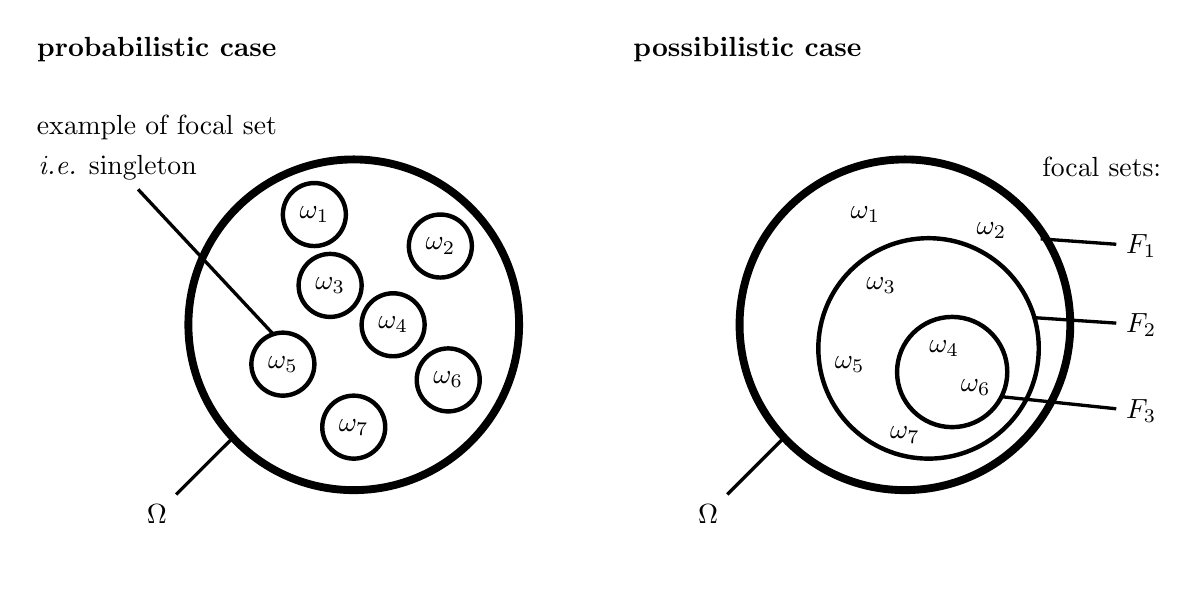
\begin{tikzpicture}
\draw[line width=1mm] (0,2) circle (2.1cm);
\node at (-0.5  , 3.4) {$\omega_1$};
\node at (1.2, 1.3) {$\omega_6$};
\node at (1.1, 3) {$\omega_2$};
\node at (0  , 0.7) {$\omega_7$};
\node at (0.5  , 2) {$\omega_4$};
\node at (-0.9  , 1.5) {$\omega_5$};
\node at (-0.3  , 2.5) {$\omega_3$};
\draw[ultra thick] (-0.5  , 3.4) circle (0.4cm);
\draw[ultra thick] (1.2, 1.3) circle (0.4cm);
\draw[ultra thick] (1.1, 3) circle (0.4cm);
\draw[ultra thick] (0  , 0.7) circle (0.4cm);
\draw[ultra thick] (0.5  , 2) circle (0.4cm);
\draw[ultra thick] (-0.9  , 1.5) circle (0.4cm);
\draw[ultra thick] (-0.3  , 2.5) circle (0.4cm);
\node (omegasetPROB) at (-1.4 , 0.7) {};
\node (omegaPROB) at (-2.5 , -0.4) {$\Omega$};
\draw[very thick] (omegasetPROB) -- (omegaPROB);
\node (FSsetPROB) at (-0.9 , 1.75) {};
\node (FSPROB) at (-2.5 , 5.5) {\textbf{probabilistic case}};
\node (FSPROB) at (-2.5 , 4.5) {example of focal set}; 
\node (FSPROB) at (-3 , 4) {\textit{i.e.} singleton};
\draw[very thick] (FSsetPROB) -- (FSPROB);

\draw[line width=1mm] (7,2) circle (2.1cm);
\draw[ultra thick] (7.3,1.7) circle (1.4cm);
\draw[ultra thick] (7.6,1.4) circle (0.7cm);
\node at (6.5  , 3.4) {$\omega_1$};
\node at (7.9, 1.2) {$\omega_6$}; %2
\node at (8.1, 3.2) {$\omega_2$}; %3
\node at (7  , 0.6) {$\omega_7$};%4
\node at (7.5  , 1.7) {$\omega_4$};%5
\node at (6.3  , 1.5) {$\omega_5$};%6
\node at (6.7  , 2.5) {$\omega_3$};%7
\node (omegasetPI) at (5.6 , 0.7) {};
\node (omegaPI) at (4.5 , -0.4) {$\Omega$};
\draw[very thick] (omegasetPI) -- (omegaPI);
\node (FSPI) at (5 , 5.5) {\textbf{possibilistic case}};
\node at (9.5, 4) {focal sets:};
\node (FSPI1) at (10, 3) {$F_1$};
\node (FSPI2) at (10, 2) {$F_2$};
\node (FSPI3) at (10, 0.9) {$F_3$};
\node (FSsetPI1) at (8.6 , 3.1) {};
\node (FSsetPI2) at (8.5 , 2.1) {};
\node (FSsetPI3) at (8.1 , 1.1) {};
\draw[very thick] (FSsetPI1) -- (FSPI1);
\draw[very thick] (FSsetPI2) -- (FSPI2);
\draw[very thick] (FSsetPI3) -- (FSPI3);


\node at (0,-1) {};
\end{tikzpicture}
\caption[Focal sets of a probability measure and a possibility measure]
{The focal sets of a mass function $m:2^{\Omega} \rightarrow [0,1]$ 
are the subsets $A \subseteq \Omega$ of the universe 
$\Omega = \set{ \omega_1,\ldots,\omega_7}$
such that the mass function is positive: $m(A)>0$.
As Probability Theory and Possibility Theory
are particular cases of BFT (see Figure \ref{uncertainty_theories}),
each of the probability (resp. possibility) distributions
is equivalent to certain mass function.
Thus, the left part of the illustration 
shows the focal sets 
from a probability measure $\mathbb{P}$:
they are the singletons of $\Omega$
and $m(\set{\omega}) = \mathbb{P}( \set{\omega} )$. 
The right part shows the focal sets 
from a possibility measure: they are nested subsets of $\Omega$,
denoted by $F_3 \subset F_2 \subset F_1 = \Omega$.}
\label{figure_focalsets}
\end{figure}



%%%%%%%%%%%%
% POSS QUAL
\subsection*{Possibility Theory}
A possibility measure has been defined 
as the plausibility measure 
of a mass function $m$
whose focal sets are nested 
(see Figure \ref{figure_focalsets}).
Let us denote these nested subsets by $F_i$, $\forall i \in \set{1,\ldots,d}$,
with $d$ a positive integer:
$F_d \subset F_{d-1} \subset \ldots \subset F_1 = \Omega$.
Note that if $A \subseteq \Omega$ and for a given $i \in \set{1,\ldots,d}$, 
$A \cap F_i \neq \emptyset$,
then $A \cap F_j \neq \emptyset$ for each $j \in \set{1,\ldots,i}$
since focal sets are nested.	
As defined in Figure \ref{uncertainty_theories},
the plausibility measure is 
$Pl(A) = \sum_{B \cap A = \emptyset} m(B)$,
$\forall A \subseteq \Omega$.
Thus, it is easy to show that for each $A \subseteq \Omega$,
$Pl(A) = \sum_{i=1}^{d_A} m(F_i)$,
where $d_A = \max \Big\{ i \in \set{1,\ldots,d} \Big\vert F_i \cap A \neq \emptyset \Big\}$.
As $d_{A \cup B} 
= \max \Big\{i \in \set{1,\ldots,d} \Big\vert F_i \cap A \neq \emptyset 
\mbox{ or } F_i \cap B \neq \emptyset \Big\}$,
this integer can be written 
$d_{A \cup B} = \max \set{d_A,d_B}$, 
and then 
\[�Pl(A \cup B) = \sum_{i=1}^{d_{A\cup B}} m(F_i) 
= \max \set{ \sum_{i=1}^{d_{A}} m(F_i), \sum_{i=1}^{d_{B}} m(F_i)  } 
= \max \Big\{ Pl(A), Pl(B) \Big\}. \]
Note also that $Pl(\Omega) = 1$ as the mass function sums to $1$ over $2^{\Omega}$,
and that $Pl(\emptyset) = 0$ as the mass function 
assigns zero to the empty set by definition.

The classical definition 
of a possibility measure, 
denoted by $\Pi: 2^{\Omega} \rightarrow [0,1]$,
is in fact the results presented just above:
\begin{itemize} 
\item $\Pi(\Omega) = 1$;
\item $\Pi(\emptyset) = 0$; 
\item $\forall A,B \subseteq \Omega$, $\Pi(A \cup B) = \max \Big\{ \Pi(A), \Pi(B) \Big\}$.
\end{itemize}
It follows that this measure is entirely 
defined by the associated possibility distribution,
\textit{i.e.} the possibility measure of the singletons: 
$\forall \omega \in \Omega$, $\pi(\omega) = \Pi(\set{\omega})$. 
Indeed, the possibility value 
of a given event
can be defined as
the maximal possibility value 
of the elementary events 
constituting the event of interest:
$\Pi(A) = \max_{\omega \in A} \pi(\omega)$.
This is quite similar 
to the fact that 
a probability measure 
over the finite universe $\Omega$,
$\mathbb{P}: 2^{\Omega} \rightarrow [0,1]$,
is equivalent to the associated
probability distribution 
$\textbf{p}: \omega \mapsto \mathbb{P}(\set{\omega})$,
using the additivity of the probability measure.

The definition of this measure lead to
the possibilistic normalization: 
\begin{equation*} 
\max_{\omega \in \Omega} \pi(\omega) = \Pi(\Omega) = 1.
\end{equation*}
If $(\overline{\omega},\underline{\omega}) \in \Omega^2$ 
are such that $\pi(\overline{\omega})<\pi(\underline{\omega})$, 
the meaning is that $\overline{\omega}$ 
is less plausible than $\underline{\omega}$. 
Elementary events with possibility degree $0$, 
\textit{i.e.} $\omega \in \Omega$ 
such that $\pi(\omega)=0$, are impossible
(same meaning as $\textbf{p}(\omega)=0$, 
with $\textbf{p}:\Omega \rightarrow [0,1]$ 
a probability distribution).
Moreover, elementary events 
such that $\pi(\omega)=1$ 
are entirely possible.

As $\Omega$ is a finite set,
the number of possible values
of a possibility distribution
is finite 
(much like a probability distribution
over a finite universe $\Omega$):
let us denote by 
$\set{ l_1,l_2,\ldots,0 }$ with
$1=l_1>l_2>\ldots>0$, 
the different values 
of the possibility distribution,
\textit{i.e.} $\set{ \pi(\omega) \sachant \omega \in \Omega }$.

On the one hand, if the current 
possibilistic belief 
coincide with the distribution
$\pi(\omega)=1$, 
$\forall \omega \in \Omega$, 
all elementary events are totally possible,
and it models therefore 
the total ignorance 
of the actual elementary event:
this means that 
Possibility Theory can 
encode agent ignorance,
one of the issues 
guiding our work.
On the other hand, 
the full knowledge 
of the actual elementary event, 
say $\tilde{\omega} \in \Omega$,
is encoded by a possibility distribution 
equal to the classical indicator function 
of the singleton 
$\set{ \tilde{\omega} }$, \textit{i.e.} 
$\pi(\omega) 
= \mathds{1}_{\set{ \tilde{\omega} }}(\omega)$.

Finally, between these two extrema, 
a possibilistic situation 
is described by
a set of entirely 
possible elementary events, 
$\set{ \omega \in \Omega 
\mbox{ s.t. } \pi(\omega)=1 }$,
and successive sets of less plausible 
ones $\set{ \omega \in \mathcal{S} \mbox{ s.t. } \pi(\omega)=l_i}$
down to the set of impossible states 
$\set{ \omega \in \Omega \mbox{ s.t. } \pi(\omega)=0  }$.

As already explained 
(see above and Figure \ref{uncertainty_theories}),
a remnant from BFT is the existence of
two measures in Possibility Theory:
the first one is the possibility measure, 
denoted by $\Pi$,
and called plausibility measure in BFT ($Pl$).
The second one is the necessity measure, 
denoted by $\mathcal{N}$,
and called belief measure in BFT ($bel$).
Recall that, given a mass function $m$,
the belief measure of the set $A \subseteq \Omega$
is $bel(A) = \sum_{B \subseteq A} m(B)$.
Now, if the mass represents a situation
which can be expressed with Possibility Theory, 
the focal sets $(F_i)_{i=1}^d$ 
of the mass function are nested:
$F_d \subset F_{d-1} \subset \ldots \subset F_1 = \Omega$
with $d \in \mathbb{N}^*$ 
the number of focal sets.
Note that if $F_i \subseteq A$ 
for a given $i \in \set{1, \ldots,d}$,
$F_j \subseteq A$, 
$\forall j \geqslant i$,
because focal sets are nested.
Thus, given $A \subseteq \Omega$, 
a distinction is made
between two cases.

The first case is when $F_d \not\subseteq A$:
in this case $bel(A) = 0$
since no focal set is in $A$.
Let us denote by $\overline{A}$ the complementary set of $A$:
$A \cup \overline{A} = \Omega$ and $A \cap \overline{A} = \emptyset$.
Now an obvious remark about sets is recalled: 
if $A$ and $B$ are two subsets of $\Omega$,
``$B \subseteq A$'' $\Leftrightarrow$ ``$B \cap \overline{A} = \emptyset$''.
Hence, in the first case, $\overline{A} \cap F_i \neq \emptyset$
for each $i \in \set{1,\ldots,d}$, 
and then the plausibility of $\overline{A}$ 
is $Pl(\overline{A}) = 1$
(as the sum of all focal sets).
So, in this case, $Pl(\overline{A}) + bel(A) = 1$.
 
In the second case, \textit{i.e.} $F_d \subseteq A$ (and thus $A \neq \emptyset$),
it is easy to show that
$bel(A) = \sum_{i=d^A}^{d} m(F_i)$,
where $d^A = \min \Big\{ i \in \set{1,\ldots,d} \Big\vert F_i \subseteq A \Big\}$.
Thus, if $A \neq \Omega$, we can see that
$ \min \Big\{ i \in \set{1,\ldots,d} \Big\vert F_i \cap \overline{A} = \emptyset \Big\}
= 1 + \max \Big\{ i \in \set{1,\ldots,d} \Big\vert F_i \cap \overline{A} \neq \emptyset \Big\}$
\textit{i.e.} $d^A = 1+d_{\overline{A}}$ (thanks to the obvious remark about sets),
where $d_A$ is defined above as 
$\max \Big\{ \set{ 1,\ldots,d } \Big\vert F_i \cap A \neq \emptyset \Big\}$.
As shown above, 
$Pl(\overline{A}) = \sum_{i=1}^{d_{\overline{A}}} m(F_i)$,
thus if $A \neq \Omega$, $Pl(\overline{A}) + bel(A) = 1$.
Finally, if $A = \Omega$, all the focal sets are included in $A$,
so $bel(A)=1$, and $\overline{A} = \emptyset$,
so $Pl(\overline{A})=0$:  $Pl(\overline{A}) + bel(A) = 1$ too.

That is why the necessity measure, 
which corresponds to the belief measure $bel$ in BFT, 
can be defined from the possibility measure as follows: 
$\forall A \subseteq \Omega$,
\[ \mathcal{N}(A) = 1 - \Pi(\overline{A}). \]

Note that we can differentiate 
Quantitative Possibility Theory \cite{Du2006.7}
from Qualitative Possibility Theory \cite{DBLP:journals/eor/DuboisPS01}.
The former uses the product 
when combining possibility distributions
in order to compute joint distributions
(much like in Probability Theory).
The latter uses 
the $\min$ operator 
for this purpose
(see Section \ref{qualitative_indep} 
of Chapter \ref{chap_SOTA}).
Thus, the qualitative theory 
uses only $\max$ and $\min$ operators.
Consider some
possibility distributions
whose values are in the finite set 
$\set{ l_1,l_2,\ldots,0 }$:
as only $\max$ and $\min$ operators 
are allowed, 
computations do not generate
any value not already included 
in the finite set $\set{ l_1,l_2,\ldots,0 }$.
This is not true for 
Quantitative Possibility Theory
since the use of the product operator 
leads to the creation 
of new real values in $[0,1]$. 

Finally, in the qualitative framework, 
the possibility values 
assigned to each of the elementary events 
are not really taken into account
in terms of real numbers
since only qualitative comparisons 
are performed via the use of 
$\max$ and $\min$ operators.
Hence, Qualitative Possibility Theory
is classically defined 
with the introduction of
a qualitative scale $\mathcal{L}$,
which may be defined as $\set{l_1,l_2,\ldots,0 }$,
or as any other totally ordered set indifferently.
As they are qualitative data, 
we use the term \textit{possibility degrees} 
instead of possibility values.
Next section clarifies why 
the use of a qualitative framework
is beneficial in terms of complexity
and modeling.

Note the similarities between 
Possibility and Probability Theory, 
replacing $\max$ by $+$, and $\min$ by $\times$
(in the qualitative case). 
Note also that Qualitative 
Possibility Theory defines
the semiring $(\mathcal{L},\max,\min)$,
and Quantitative Possibility Theory
leads to the semiring $([0,1]\max,\times)$.
These algebraic structures are
close to the well known 
tropical semirings \cite{pin:hal-00113779},
as the \textit{max-plus} semiring 
$(\mathbb{R} \cup \set{-\infty} \max,+)$ 
and the \textit{min-plus} one 
$(\mathbb{R} \cup \set{+\infty}, \min,+)$.

%%% PIPOMDP
\subsection*{Qualitative Possibilistic POMDP}
A qualitative possibilistic counterpart 
of the POMDP framework
has been proposed in \cite{Sabbadin:1999:pipomdp}:
this model is called Qualitative Possibilistic POMDP 
and denoted by $\pi$-POMDP. 
A $\pi$-POMDP is simply a POMDP
with qualitative possibility distributions as parameters,
instead of probability distributions.
As the $\pi$-POMDP framework is qualitative,
the counterpart of the reward function,
called \textit{preference function},
is a qualitative function: 
indeed the preference function returns values 
from the finite qualitative scale $\mathcal{L}$,
and thus is non-additive.

%%IMPRECISION CRITERES
As a particular case of BFT
and \textit{a fortiori} of IPT,
Possibility Theory expresses 
a partial knowledge
of the actual probability distribution,
as presented above.
A qualitative possibility distribution
is even more imprecise
since only qualitative information
is given by such a distribution.
This imprecision results in the measures
presented above: possibility and necessity measures. 
As detailed in Section \ref{subsection_qualcrit},
two qualitative criteria have been proposed 
in \cite{DBLP:journals/ijar/SabbadinFL98},
counterparts of the probabilistic criterion (\ref{criterion}): 
a pessimistic one, which is a
qualitative counterpart of the maximin 
(worst-case) criterion in IPT.
The other criterion qualifies as optimistic, 
as a qualitative counterpart of 
the best case criterion in IPT.

%%%% COMPLEXITY 
One of the most interesting property
of the $\pi$-POMDPs is
the simplification of the strategy computation.
Indeed, algorithms proposed 
for solving classical (probabilistic) POMDPs
are often based on the set of the belief states
called \textit{belief space}.
The belief space is infinite in the general case: 
each time step leads eventually 
to a finite number of new belief states,
which makes this set countable. 
In order to get useful properties
for the strategy computation,
the set of all probability distributions
over the system space $\mathcal{S}$ is considered, 
\textit{i.e.} the continuous simplex
$\mathbb{P}^{\mathcal{S}} 
= \set{ \textbf{p}:\mathcal{S} \rightarrow [0,1] \sachant \sum_{s \in \mathcal{S}} \textbf{p}(s) 
= 1, \mbox{ and } \textbf{p}(s)\geqslant 0, \forall s \in \mathcal{S} }$.
The infinite size of the belief space 
partly explains why probabilistic POMDPs
are very hard to resolve.
On the contrary, $\pi$-POMDPs have a finite belief space.
Indeed, the number of qualitative possibility distributions
over the system space $\mathcal{S}$
is lower than $\mathcal{L}^{\# \mathcal{L}}$,
as the qualitative scale $\mathcal{L}$ is finite.
The fully observable version 
of the $\pi$-POMDP model is called $\pi$-MDP:
as explained in Section \ref{section_piPOMDP} of Chapter \ref{chap_SOTA}, 
any $\pi$-POMDP reduces to a $\pi$-MDP whose system space is
the qualitative possibilistic belief space, and
whose size is exponential in the number of states.
In works \cite{DBLP:journals/corr/abs-1202-3718,Garcia20081018,Sabbadin:1999:pipomdp}, 
$\pi$-MDP complexity appears to be lower than MDP complexity, which is polynomial \cite{Papadimitriou:1987}:
$\pi$-POMDP complexity is then
at worst exponential in the process description,
whereas POMDP solving may be undecidable \cite{Madani:1999:UPP:315149.315395}.
The approach of using of a $\pi$-POMDP instead of a probabilistic POMDP
in order to simplify the resolution, can be compared to 
the \textit{Predictive State Representation} approach \cite{Littman01predictiverepresentations}:
indeed, the latter also represents the agent knowledge in a more compact way.

%%% IMPRECISION MODELISATION
In addition to the simplification of the computations,
the $\pi$-POMDP framework may be very interesting for modeling.
Indeed, when we considered 
a robot using computer vision algorithms
to get observations
(see Figure \ref{observation_robot}),
we previously highlighted the difficulty
of defining properly 
the probabilistic observation function:
probability values of the answers
of the vision algorithms
in the context of the robotic mission
are imprecisely known 
and hard to define in practice.
Finding qualitative estimates 
of their recognition performance is easier: 
the $\pi$-POMDP model 
only requires qualitative data, 
thus it allows to build the model 
without the use of information 
other than the one really available. 
For instance, 
the confusion matrix 
in Figure \ref{confusion_matrix}
may lead to a qualitative possibilistic 
observation function 
which only takes into account
how answer frequencies are sorted:
in the presence of a human (see second line),
the most frequent answer is ``human'',
the second one is ``nothing'',
the third one is ``car'', etc.
Thus, the corresponding possibility distribution
is such that, 
conditional on the presence of a human,
the possibility degree 
of the answer ``human''
is higher than the possibility degree 
of the answer ``nothing'',
which is higher than the possibility degree 
of the answer ``car'', etc.
Instead of assigning frequencies 
which are not really reliable in practice, 
the qualitative possibilistic model
naturally expresses imprecisions
about the problem.

%%%IGNORANCE
Finally, let us recall that 
the constant possibility distribution
whose possibility degrees are all equal to $1$ 
(maximal element of $\mathcal{L}$),
represents total ignorance: 
this distribution can be used 
to define the initial belief state
when it has to represent 
an agent which initially ignores
a given situation.
Thus, the $\pi$-POMDP framework 
allows a formal modeling 
of the agent's lack of knowledge.

%%CORRESPONDS TO OUR ISSUES 
The use of the Qualitative Possibility Theory 
\cite{DBLP:journals/eor/DuboisPS01}
is thus studied in this work,
as it appears able
to both simplify a POMDP, 
and model parameter imprecision 
and ignorance
related to robotic missions.
This framework indeed simplifies computations,
is able to encode the problem with only available data
and formally models the lack of knowledge:
thus this theory offers solutions to
the three issues highlighted previously.
However we note that, as a qualitative framework, 
it does not allow 
frequentist information encoding.

%%%NOT WIDELY STUDIED
To the best of our knowledge,
a very limited study of the $\pi$-POMDP model
exists in the literature up to now:
in fact, the work \cite{Sabbadin:1999:pipomdp}
seems to be the only one proposing 
both a definition of the $\pi$-POMDP
and a toy example to illustrate this model.
The fully observable version ($\pi$-MDP)
has generated some more interest
\cite{Sabbadin2001287,conf/ecai/Sabbadi00,LIP61498}.

\section*{Description of our Study}
% Le sujet de la th�se
This thesis contributes to determine
what Qualitative Possibility Theory 
can provide in \textit{planning under uncertainty
in partially observable domains}, 
and more generally in 
\textit{sequential uncertainty management}, 
in terms of computation simplification 
and modeling. 
It presents recent contributions 
in the use of this theory
for planning under uncertainty 
and knowledge representation,
with an almost systematic use of 
graphical models 
\cite{Koller:2009:PGM:1795555,Be2002.7,Borgelt02graphicalmodels}.

The end of this introduction describes how this thesis is structured.
Indeed, each of the following sections 
corresponds to a chapter of our work
and details its contents.

%%%% SOTA
\subsection*{State of the art}
As the probabilistic POMDP and the qualitative possibilistic one 
are the central objects of this thesis,
the \emph{first chapter} presents these models
starting from low level definitions.
Most of the classical results presented 
are accompanied by proofs
making this thesis self-contained:
this work is thus accessible 
to all researchers 
and students
with basic mathematical competences, 
even if they are not familiar 
with alternative uncertainty theories,
nor member of the \textit{planning under uncertainty} community.

The first part of this chapter focuses on
the classical (probabilistic) POMDP:
it begins with the presentation of the less complex 
fully observable case, called MDP.
The well-know POMDP is then set up, 
giving some formal results and proofs 
hard to find in the literature. 
This part ends with a review 
of a large part 
of the successful POMDP algorithms
including the ones used in the next chapters. 

The second part is naturally devoted to
the qualitative possibilistic counterpart of the POMDP.
It begins with a presentation of the Possibility Theory,
with a specific focus on the qualitative version.
It includes the qualitative counterparts of conditioning,
and averaging.
Finally, as all the needed theoretical tools have been presented,
the fully observable model ($\pi$-MDP) can be defined,
followed by the partially observable one ($\pi$-POMDP).
As noted above, to the best of our knowledge,
only one ten-paged paper has already dealt with
the $\pi$-POMDPs: 
the second part of this chapter is thus the first work 
detailing formally the construction of this model.

Note that the notations and the terminology 
set up in this initial chapter,
and thus used throughout this thesis,
are those classically used in the POMDP framework:
it should make our work more readable to the POMDP community 
or more generally to the probabilistic community.
Moreover, dedicating 
this first chapter 
to a formal presentation of 
the probabilistic and the qualitative possibilistic models
is meant to highlight their common structure.

%%% CHAP1
\subsection*{Natural updates of the possibilistic model}
The \emph{second chapter} proposes several extensions 
of the work \cite{Sabbadin:1999:pipomdp}.
It begins with the presentation of some variants 
of the qualitative criteria presented in the first chapter:
the latter are related to the aggregations of the preferences over time,
and to the chosen approach \textit{i.e.} pessimistic or optimistic.

A qualitative possibilistic version of the
Mixed-Observable MDPs 
\cite{OngShaoHsuWee-IJRR10,AraThoBufCha-ICTAI10}, 
named $\pi$-MOMDP and generalizing both $\pi$-MDP and $\pi$-POMDP,
is then built: 
it reduces dramatically 
the complexity of solving $\pi$-POMDPs, 
some state variables of which are fully observable. 
For instance, the battery level of a robot
may be considered as directly 
exploitable for the decision,
making computations easier.
More generally, the existence of visible variables 
is common in robotics \cite{OngShaoHsuWee-IJRR10}.

Next, a qualitative criterion
for missions with unbounded durations
is proposed, along with
an algorithm for computing the associated
optimal strategy.
This algorithm is used to
compute a strategy 
for a target recognition mission:
experimental results compare 
executions using this strategy to
those using the strategy from a probabilistic algorithm, 
in situations where the probabilistic dynamic of the observations 
is not properly defined.

Note that this experiment is the first practical use
of the $\pi$-POMDP framework.
It also highlights interesting behaviors
of the qualitative possibilistic belief state:
they are then clarified theoretically 
in the end of the chapter.

The main contributions of this chapter 
have been published in \cite{Drougard13}.
The experiment illustrates that 
these contributions are necessary in practice.
However they are not sufficient
to reach a competitive computation time
or to deal with realistic robotic problems:
the orientation of the next chapter
stems from this observation.

%%% CHAP2
\subsection*{Factorized models and symbolic algorithms}

%% INTRO
The size of the robotic problem dealt with 
in the previous chapter
is small enough to allow the proposed algorithm 
to compute a strategy within a reasonable amount of time.
The contributions of the \emph{third chapter}
are meant to make computations possible 
for larger structured planning problems. 

%% PPUDD and factored models
The first part of this chapter 
proposes a definition 
for the \textit{factored $\pi$-MOMDPs}:
additional independence assumptions 
are provided to these processes --
in a qualitative possibilistic sense,
as defined in the first chapter.
Large planning problems satisfying these assumptions 
can be solved more easily:
building upon the probabilistic 
SPUDD algorithm \cite{Hoey99spudd:stochastic},
we conceived an algorithm named PPUDD 
for solving factorized $\pi$-MOMDPs
using \textit{Algebraic Decision Diagrams} (ADD).
The guess motivating this contribution 
is that computations between ADDs 
is less time and memory consuming
when performed in the possibilistic framework 
than in the probabilistic one:
qualitative operations
should lead to smaller ADDs
when sum and product
produce ADDs with potentially
more leaves.

%% belief factorization
Independence assumptions defining 
a factored $\pi$-MOMDP 
concerns the variables encoding 
successive belief states.
However variables defining a factored $\pi$-MOMDP
are those representing 
successive system states and observations.
That is why, the following section
of this chapter exhibits sufficient conditions 
on the system state and observation variables
leading to the desired independence 
between belief state variables.
A robotic example is used as an illustration
of these conditions.
As proofs use the graphical concept 
called \textit{$d$-Separation} \cite{pearl88},
these conditions also lead to the
belief variable independence 
in the probabilistic MOMDP framework.
 
%% first tests, larger robotic missions TODO TODO 
Performances of our solver PPUDD 
are next compared to
those of its probabilistic counterparts, 
in terms of computation time, 
and with criteria measuring 
the mission achievement. 
Finally, the last part of this chapter
describes the results of PPUDD 
at the International Probabilistic 
Planning Competition\footnote{\url{https://cs.uwaterloo.ca/~mgrzes/IPPC_2014/}}.
We participated in the competition
in order to test the performances
of our algorithm
against probabilistic one,
in terms of expected reward,
with various
probabilistic planning problems. 

%% CITE PUBLI
Some contributions of this chapter 
have been published in 
\cite{DBLP:conf/aaai/DrougardTFD14}.
%% ISSUES, link with the next (model -> HMI / model+ADD -> hybrid)
The various planning problems
of the competition also highlight 
some issues of our algorithm
when used to find an approximate strategy
for a probabilistic problem
in order to
benefit from qualitative computations
which are simpler.
Although modeling points are part of these issues,
the next chapter shows that 
a possibilistic approach
is very useful 
where only qualitative
data are available.
The approach proposed in the final chapter 
takes into account 
the highlighted modeling issues.
Moreover, time can be lost 
before computations of PPUDD,
when loading ADDs encoding some 
high dimensional planning problems:
memory issues are also observed in practice.
Hence the last chapter focuses on 
the belief state management
as MDP algorithms using state space search
\cite{DBLP:conf/aips/KellerE12,DBLP:conf/aaai/KolobovMW12} 
do not face these issues
and can solve the problem resulting 
from this last step of the study.

%%% CHAP3
\subsection*{A qualitative possibilistic process for human-machine interaction modeling}
%%% why? qualitative info only
The \emph{fourth chapter} deals with
situations where probability distributions
are clearly not available:
the managed problem comes from the work
\cite{SERGIOTHESIS} and is a joint work with the author,
Sergio Pizziol, working on the field of 
\textit{Human-Machine Interactions} (HMI).
In systems representing human behavior 
in certain situations,
for instance interacting with a control panel
of an aerial vehicle,
a sufficient amount of statistical data is lacking,
especially concerning the human operator's state of mind:
only expert knowledge can be used in practice
as no frequentist information about the problem
is available.

%% like with previous processes
In this chapter, used processes 
are similar to those
studied in the previous chapters:
the only difference is that actions 
are not chosen anymore, but used as observations
to infer the state of the human-machine system.
This process is called \textit{qualitative possibilistic Hidden Markov Process}
($\pi$-HMP).

This process is used as a tool
to produce diagnosis for
HMI systems: machine state 
and human actions are called \textit{occurrences},
and the possible transitions of the system
are called \textit{effects}.
After the model construction 
describing the problem in terms
of occurrences and effects
from expert qualitative data
and the machine model,
the human assessment of the situation can be estimated.
The proposed model can also detect
human assessment errors, 
and produce a diagnosis for them.

%%% CHAP4
\subsection*{Probabilistic-possibilistic approach: a hybrid perspective}
The last chapter of this thesis
persists to show the possible 
improvement of the POMDP framework
using the qualitative possibility theory,
especially for the belief state management.
It also takes into account the issues
highlighted in the third chapter.

Indeed, the \emph{fifth chapter} 
argues for a hydrid POMDP 
with both probabilistic 
and possibilistic settings. 
A new translation from Partially Observable MDP 
into Fully Observable MDP is described here. 
Unlike the classical translation
presented in the first chapter, 
the resulting problem state space is finite, 
making probabilistic MDP solvers able to solve
this simplified version 
of the initial partially observable problem.
Indeed, this approach encodes agent beliefs 
with possibility distributions over states,
leading to an MDP whose state space 
is a finite set of epistemic states.

Additional simplifications of the computations
are described for \textit{factored POMDPs} \cite{Sim:2008:SHS:1620163.1620241,Williams05factoredpartially,
Veiga14aaai,DBLP:journals/corr/abs-1301-6719}, \textit{i.e.}
POMDPs with a particular independence 
structure.
These last contributions have been published in
\cite{DBLP:conf/sum/DrougardDFT15}.
